\documentclass[11pt,a4paper]{article}

\usepackage[margin=2.4cm]{geometry}
\usepackage{amsmath,amssymb}
\usepackage{graphicx}
\usepackage{booktabs}
\usepackage{float}
\usepackage[font=small,labelfont=bf]{caption}
\usepackage{xcolor}
\usepackage{microtype}
\usepackage[colorlinks=true,linkcolor=blue!50!black,urlcolor=blue!50!black,citecolor=blue!50!black]{hyperref}

\graphicspath{{../results/figures/}}
% AUTO-GENERATED by report/make_tables.py -- do not edit by hand.
\newcommand{\pendTableRows}{%
DMD & 0.624 & $1.10$ & $0.5$ & 0\% & $3.9\times10^{-2}$ \\
EDMD & 0.064 & $\geq 12.00$ & $\geq 6.0$ & 87\% & $1.4\times10^{-6}$ \\
Deep Koopman & 0.197 & $6.12$ & $3.1$ & 7\% & $2.5\times10^{-2}$ \\
}
\newcommand{\lorenzTableRows}{%
DMD & 1.066 & 0.05 & 0.05 & 0\% & $1.0\times10^{0}$ \\
EDMD & 0.782 & 0.20 & 0.21 & 0\% & $1.1\times10^{-3}$ \\
Deep Koopman & 0.952 & 0.44 & 0.44 & 0\% & $7.8\times10^{-1}$ \\
}
\newcommand{\ladderTableRows}{%
reconstruction (no dynamics) & 0.024 \\
1 step ahead & 0.072 \\
1 Lyapunov time & 0.627 \\
3 Lyapunov times & 1.194 \\
}
\newcommand{\pendNTrain}{60}
\newcommand{\pendNVal}{12}
\newcommand{\pendNTest}{30}
\newcommand{\pendDamping}{0.2}
\newcommand{\pendDt}{0.05}
\newcommand{\pendTfinal}{12}
\newcommand{\pendDKLatent}{16}
\newcommand{\pendDKHorizon}{60}
\newcommand{\pendDKIter}{4000}
\newcommand{\pendEDMDK}{4}
\newcommand{\pendEDMDP}{5}
\newcommand{\pendEDMDFeatures}{55}
\newcommand{\lorNTrain}{10000}
\newcommand{\lorNVal}{2000}
\newcommand{\lorNTest}{4000}
\newcommand{\lorNStarts}{46}
\newcommand{\lorDt}{0.02}
\newcommand{\lorDKLatent}{32}
\newcommand{\lorDKHorizon}{40}
\newcommand{\lorDKIter}{3000}
\newcommand{\lorEDMDDegree}{4}
\newcommand{\lorEDMDFeatures}{34}


\newcommand{\R}{\mathbb{R}}
\newcommand{\C}{\mathbb{C}}
\newcommand{\Kop}{\mathcal{K}}
\newcommand{\norm}[1]{\left\lVert #1\right\rVert}
\newcommand{\code}[1]{\texttt{#1}}
\setlength{\parskip}{0.45em}
\setlength{\parindent}{0pt}

\title{\textbf{Koopman Operator Learning for Nonlinear Dynamics}\\[0.3em]
\large DMD, EDMD and Deep Koopman on the Nonlinear Pendulum and the Lorenz Attractor}
\author{}
\date{October 2026}

\begin{document}
\maketitle

\begin{abstract}
\noindent
This report documents a Python library that applies Koopman operator theory to nonlinear dynamical
systems. It contains custom ODE solvers for data generation, exact Dynamic Mode Decomposition (DMD)
computed through the SVD, Extended DMD (EDMD) with physics-informed observables, and a PyTorch Deep
Koopman autoencoder that learns a latent space with linear dynamics, together with visualization
tools and a test suite. The three methods are compared on a damped nonlinear pendulum (a system
with a stable equilibrium and amplitude-dependent oscillation frequency) and on the chaotic Lorenz
attractor, always by \emph{predicting} from a single initial state on held-out data. Besides the
results, the report explains how to read every figure that the code produces.
\end{abstract}

\tableofcontents
\newpage

%% ====================================================================================
\section{What was built}
%% ====================================================================================
The repository implements the following components. Each corresponds to a module of the
\code{koopman} package.

\begin{center}
\small
\begin{tabular}{@{}lp{9.2cm}@{}}
\toprule
\textbf{Module} & \textbf{Content}\\
\midrule
\code{solvers.py} & Explicit Euler, classical RK4 and an adaptive Dormand--Prince 5(4) integrator, written from scratch.\\
\code{systems.py} & Damped nonlinear pendulum and Lorenz-63; trajectory and dataset generation.\\
\code{dmd.py} & Exact DMD via the SVD (rank truncation, eigenvalues, modes, amplitudes).\\
\code{observables.py} & Polynomial dictionary and a physics-informed trigonometric dictionary for the pendulum.\\
\code{edmd.py} & EDMD: ridge-regularised least squares in the lifted space and read-out of the state.\\
\code{deep\_koopman.py} & Autoencoder with a linear latent Koopman matrix, multi-step training, spectral stabilisation.\\
\code{metrics.py} & Normalised error curves and the \emph{valid prediction time}.\\
\code{viz.py} & All plots (consistent, colour-blind-safe style).\\
\bottomrule
\end{tabular}
\end{center}

The scripts \code{experiments/pendulum.py} and \code{experiments/lorenz.py} run the full studies
(\code{python main.py}); \code{tests/} contains the \code{pytest} suite.

\paragraph{A correction relative to the first version of the repository.}
The first version compared DMD and EDMD \emph{rollouts} (started from $x_0$ only) with the
\emph{reconstruction} of the Deep Koopman autoencoder, i.e.\ $\mathrm{decode}(\mathrm{encode}(x_t))$
evaluated at every true state $x_t$. That reconstruction never uses the learned dynamics, so it
shows how well an autoencoder compresses points of the attractor, not how well the model predicts.
The statement that Deep Koopman ``nearly overlaps'' the true attractor was therefore not a
prediction result. In this version every method is evaluated in the same way: from the initial state
only, rolled forward with its own dynamics, on held-out data. The reconstruction error is still
reported, but separately (Figure~\ref{fig:ladder}).

%% ====================================================================================
\section{Theory}
%% ====================================================================================
\subsection{The Koopman operator}
Consider a flow $\dot x=f(x)$ on $\R^d$ with time-$t$ map $\varphi^t$, or a discrete map
$x_{k+1}=F(x_k)$ (for us $F=\varphi^{\Delta t}$). For an \emph{observable}, i.e.\ a scalar function
$g$ of the state, the Koopman operator acts by composition,
\begin{equation}
  (\Kop g)(x) = g\bigl(F(x)\bigr).
\end{equation}
$\Kop$ is \emph{linear} even when $F$ is nonlinear, because $\Kop(a g_1+b g_2)=a\,\Kop g_1+b\,\Kop g_2$;
the price is that it acts on an infinite-dimensional space of functions
\cite{Koopman1931,Brunton2022}. If $\Kop\psi_j=\lambda_j\psi_j$ ($\psi_j$ an eigenfunction) and the
state coordinates are expanded as $x=\sum_j v_j\psi_j(x)$ with \emph{Koopman modes} $v_j$, then
\begin{equation}
  x_k=\sum_j v_j\,\lambda_j^{\,k}\,\psi_j(x_0),
\end{equation}
so the dynamics decouple into modes that grow or decay at rate $\log|\lambda_j|/\Delta t$ and oscillate at
angular frequency $\arg\lambda_j/\Delta t$. The goal of the three methods below is to find a finite-dimensional
approximation of $\Kop$ from data and to use it to predict.

\subsection{Exact DMD}
Given snapshot pairs $(x_k,y_k=F(x_k))$ arranged as columns of $X,Y\in\R^{d\times m}$, DMD finds the
best linear operator $A=YX^{\dagger}$ and its spectrum \cite{Schmid2010,Tu2014}. With the thin SVD
$X=U\Sigma V^{*}$ truncated to rank $r$:
\begin{enumerate}
  \item reduced operator $\tilde A=U^{*}YV\Sigma^{-1}\in\R^{r\times r}$;
  \item eigendecomposition $\tilde A W=W\Lambda$;
  \item \emph{exact} DMD modes $\Phi=YV\Sigma^{-1}W$, which satisfy $A\Phi=\Phi\Lambda$;
  \item amplitudes $b=\Phi^{\dagger}x_0$ and prediction $x_k=\operatorname{Re}\bigl(\Phi\Lambda^{k}b\bigr)$.
\end{enumerate}
Seen from the Koopman viewpoint, DMD approximates $\Kop$ on the span of the state coordinates
$\{x_1,\dots,x_d\}$ only. This is exact if the dynamics are linear, but for a nonlinear system the span of
the coordinates is not invariant under $\Kop$, which is the reason DMD struggles on both benchmarks.
The continuous-time spectrum is $\omega_j=\log(\lambda_j)/\Delta t$; its real part is a growth rate and its
imaginary part an angular frequency.

\subsection{Extended DMD}
EDMD enlarges the function space \cite{Williams2015}. A \emph{dictionary} of $p$ observables
$\psi(x)=[\psi_1(x),\dots,\psi_p(x)]$ (a row vector) lifts the state, and $K\in\R^{p\times p}$ is fitted
by ridge-regularised least squares over all pairs,
\begin{equation}
  K=\arg\min_{K}\ \sum_{k}\norm{\psi(y_k)-\psi(x_k)K}^2+\lambda m\norm{K}_F^2 .
\end{equation}
For $g=\psi a$ one has $\Kop g\approx\psi\,(Ka)$. The state is read back through a linear read-out
$B$ with $x\approx\psi(x)B$ (fitted by least squares; because the first $d$ features are the state itself,
$B$ simply selects them). A prediction from $x_0$ is $\hat x_k=\psi(x_0)K^{k}B$.

Feature standardisation is a diagonal similarity transform of $K$ and leaves its spectrum unchanged; it is used
only to keep the least-squares problem well conditioned. When the dictionary spans an \emph{invariant
subspace} of $\Kop$ the lifted dynamics are exactly linear. A classical example is the map
$x_1^+=\mu x_1$, $x_2^+=\lambda x_2+c\,x_1^2$, for which $\{x_1,x_2,x_1^2\}$ is invariant with eigenvalues
$\mu,\lambda,\mu^2$; the test suite checks that EDMD recovers this system to machine precision while DMD cannot.

\paragraph{Physics-informed observables for the pendulum.}
For $\ddot\theta=-\omega_0^2\sin\theta-c\dot\theta$ the dictionary uses the features
\begin{equation}
  \theta,\ \ \dot\theta,\ \ 1,\ \ \dot\theta^{\,p}\sin(k\theta),\ \ \dot\theta^{\,p}\cos(k\theta)
  \quad(p=0,\dots,P;\ k=1,\dots,N_h),\ \ \dot\theta^{\,p}\ (p=2,\dots,P).
\end{equation}
The trigonometric terms respect the $2\pi$-periodicity of the angle, and they are \emph{closed under
differentiation up to the truncation order}: $\tfrac{d}{dt}\sin\theta=\dot\theta\cos\theta$,
$\tfrac{d}{dt}\cos\theta=-\dot\theta\sin\theta$ and $\tfrac{d}{dt}\dot\theta=-\omega_0^2\sin\theta-c\dot\theta$.
Each differentiation raises the velocity degree by one, so no finite $P$ gives an exactly invariant space;
the number of harmonics $N_h$ and the velocity degree $P$ control how well it is approximated. For the Lorenz system, whose vector field is quadratic, the
dictionary is the set of monomials up to a chosen degree.

\subsection{Deep Koopman autoencoder}
Instead of choosing observables by hand, an encoder $\phi:\R^d\to\R^L$ and a decoder $\psi:\R^L\to\R^d$ are
learned jointly with a linear latent operator $K\in\R^{L\times L}$, so that $\phi(x_{k+1})\approx K\phi(x_k)$
\cite{Lusch2018}. Training uses windows $x_k,\dots,x_{k+M}$ and minimises
\begin{align}
  \mathcal L_{\mathrm{rec}} &= \bigl\|x_k-\psi(\phi(x_k))\bigr\|^2, \\
  \mathcal L_{\mathrm{lin}} &= \tfrac1M\sum_{m=1}^{M}\bigl\|\phi(x_{k+m})-K^{m}\phi(x_k)\bigr\|^2, \\
  \mathcal L_{\mathrm{pred}}&= \tfrac1M\sum_{m=1}^{M}\bigl\|x_{k+m}-\psi\bigl(K^{m}\phi(x_k)\bigr)\bigr\|^2,
\end{align}
with total loss $\mathcal L=\mathcal L_{\mathrm{rec}}+\mathcal L_{\mathrm{lin}}+\mathcal L_{\mathrm{pred}}$ (all in
standardised state units). The reconstruction term alone would let the model memorise the data without learning
any dynamics, the linearity term forces the latent space to evolve linearly, and the prediction term makes a rollout
from a single initial state meaningful. Both networks are two-hidden-layer MLPs with $\tanh$ activations; $K$ is
initialised orthogonal and trained with Adam (learning rate decayed exponentially from $2\cdot10^{-3}$ to
$10^{-4}$) with gradient clipping.

A learned $K$ can have an eigenvalue marginally outside the unit circle (e.g.\ $1.02$). This is harmless over the
short training windows but blows up in a long rollout. The method \code{DeepKoopman.stabilize} therefore rescales
only the offending eigenvalues onto the unit circle, keeping the eigenvectors; the Lorenz experiment adopts it only
if it lowers the \emph{validation} error.

%% ====================================================================================
\section{Implementation notes}
%% ====================================================================================
\paragraph{ODE solvers.}
All data come from solvers written for this project. The classical Runge--Kutta step is
\begin{equation}
  y_{n+1}=y_n+\tfrac h6\,(k_1+2k_2+2k_3+k_4),
\end{equation}
and the adaptive integrator is the Dormand--Prince embedded pair \cite{Dormand1980}: the difference of its fifth-
and fourth-order solutions estimates the local error, and the step is updated as
$h\leftarrow h\cdot\min\{10,\max\{0.2,\,0.9\,\varepsilon^{-1/5}\}\}$ with $\varepsilon$ the error scaled by
$\mathrm{atol}+\mathrm{rtol}\,|y|$. Steps are clipped so that the solution lands \emph{exactly} on the requested
output grid, so no interpolation is needed. The tests verify that Euler and RK4 converge with orders $1$ and $4$, that
the adaptive scheme meets its tolerance, that the Lorenz solution agrees with SciPy's DOP853, and that the undamped
pendulum conserves its energy to $10^{-6}$. Training data use RK4 with an internal step of at most $0.005$.

\paragraph{Test suite.}
\code{pytest} runs unit tests of each module plus short end-to-end runs of both experiments and the command-line
entry point. Notable checks: exact recovery of a linear operator and its spectrum by DMD; exact EDMD on a system
with an invariant dictionary; absence of training windows that straddle two trajectories; reproducibility with a
fixed seed; that Deep Koopman actually learns the dynamics of a linear system and generalises to unseen initial
states; and that every figure is written to disk.

%% ====================================================================================
\section{Experimental protocol}
%% ====================================================================================
\paragraph{Pendulum.} A damped pendulum with $g/L=9.81\,\mathrm{s^{-2}}$ and damping $c=\pendDamping\,\mathrm{s^{-1}}$ is
sampled every $\Delta t=\pendDt\,$s for $\pendTfinal\,$s. Initial conditions are drawn at random from a box
($|\theta_0|\le2.7$, $|\dot\theta_0|\le4$) restricted to the libration regime (energy below $95\%$ of the separatrix). There are
\pendNTrain{} training, \pendNVal{} validation and \pendNTest{} test trajectories. The small-angle period is
$2\pi/\omega_0\approx2.0\,$s, so a rollout covers about six periods.

\paragraph{Lorenz.} One long trajectory on the attractor with the classical parameters ($\sigma=10$, $\rho=28$,
$\beta=8/3$; the spin-up transient is discarded) is sampled every $\Delta t=\lorDt$. It is split
\emph{chronologically} into \lorNTrain{} training, \lorNVal{} validation and \lorNTest{} test steps, and the test
segment provides \lorNStarts{} different initial states. Since the largest Lyapunov exponent is
$\lambda_{\max}\approx0.906$, errors grow like $e^{\lambda_{\max}t}$ and time is measured in
\emph{Lyapunov times} $1/\lambda_{\max}\approx1.10$.

\paragraph{Evaluation.} Every model predicts the \emph{whole} trajectory from its initial state alone. We report
\begin{itemize}
  \item the \emph{normalised error} $e(t)=\norm{\hat x(t)-x(t)}/\sigma$, with $\sigma$ the RMS distance of the training states
        from their mean ($e=1$ is as wrong as always predicting the mean state);
  \item the \emph{mean rollout error}, the average of $e(t)$ over time and initial states;
  \item the \emph{valid prediction time}, the first time $e(t)$ exceeds $0.2$ (the median over initial states is reported);
  \item the \emph{one-step RMSE}, the error of a single application of the learned map.
\end{itemize}
\paragraph{Model selection.} All hyper-parameters are chosen on the \emph{validation} data and the test data are used once at the
end: the EDMD dictionary (harmonics $N_h\in\{1,\dots,4\}$ and velocity degree $P\in\{1,\dots,6\}$ for the pendulum; polynomial degree
$2$--$4$ for Lorenz), and for Deep Koopman the latent dimension and the prediction horizon $M$ from a small grid (documented in
the code comments of \code{experiments/}). DMD has no hyper-parameter besides its rank ($=d$).

%% ====================================================================================
\section{Results}
%% ====================================================================================

\subsection{Pendulum}
Table~\ref{tab:pend} summarises the held-out test trajectories. EDMD with the physics-informed dictionary
(\pendEDMDK{} harmonics, velocity degree \pendEDMDP{}, \pendEDMDFeatures{} observables, chosen on validation) is by far the best:
its one-step map is accurate to $10^{-6}$ and the median rollout stays below the $0.2$ threshold for the whole $12\,$s horizon.
The $\geq$ sign marks that cap: that number is a lower bound, not a measured crossing time, and the column ``never above
threshold'' gives the fraction of test runs that really never crossed it. Deep Koopman ($\pendDKLatent$-dimensional latent space,
$\pendDKHorizon$-step prediction loss, \pendDKIter{} iterations) lies in between, while plain DMD, which can only represent a
single fixed-frequency linear oscillation, loses track after about half a period.

\begin{table}[H]
\centering\footnotesize
\caption{Pendulum, held-out initial conditions, rollout from the initial state alone. The $\geq$ marks a value capped by the
$12\,$s horizon.}\label{tab:pend}
\begin{tabular}{lrrrrr}
\toprule
Method & mean error & valid time (s) & valid (periods) & never exceeded & one-step RMSE \\
\midrule
\pendTableRows
\bottomrule
\end{tabular}
\end{table}

The mechanism is visible in the amplitude sweep (Figure~\ref{fig:amp}): the pendulum's frequency drops as the amplitude grows,
which no single linear model on $(\theta,\omega)$ can reproduce, so the DMD error is large across the whole range and rises sharply for the largest amplitudes. The
dictionary of EDMD contains $\sin k\theta$ and $\cos k\theta$ terms and expresses this nonlinearity as a linear map in the lifted
space.

\begin{figure}[H]\centering
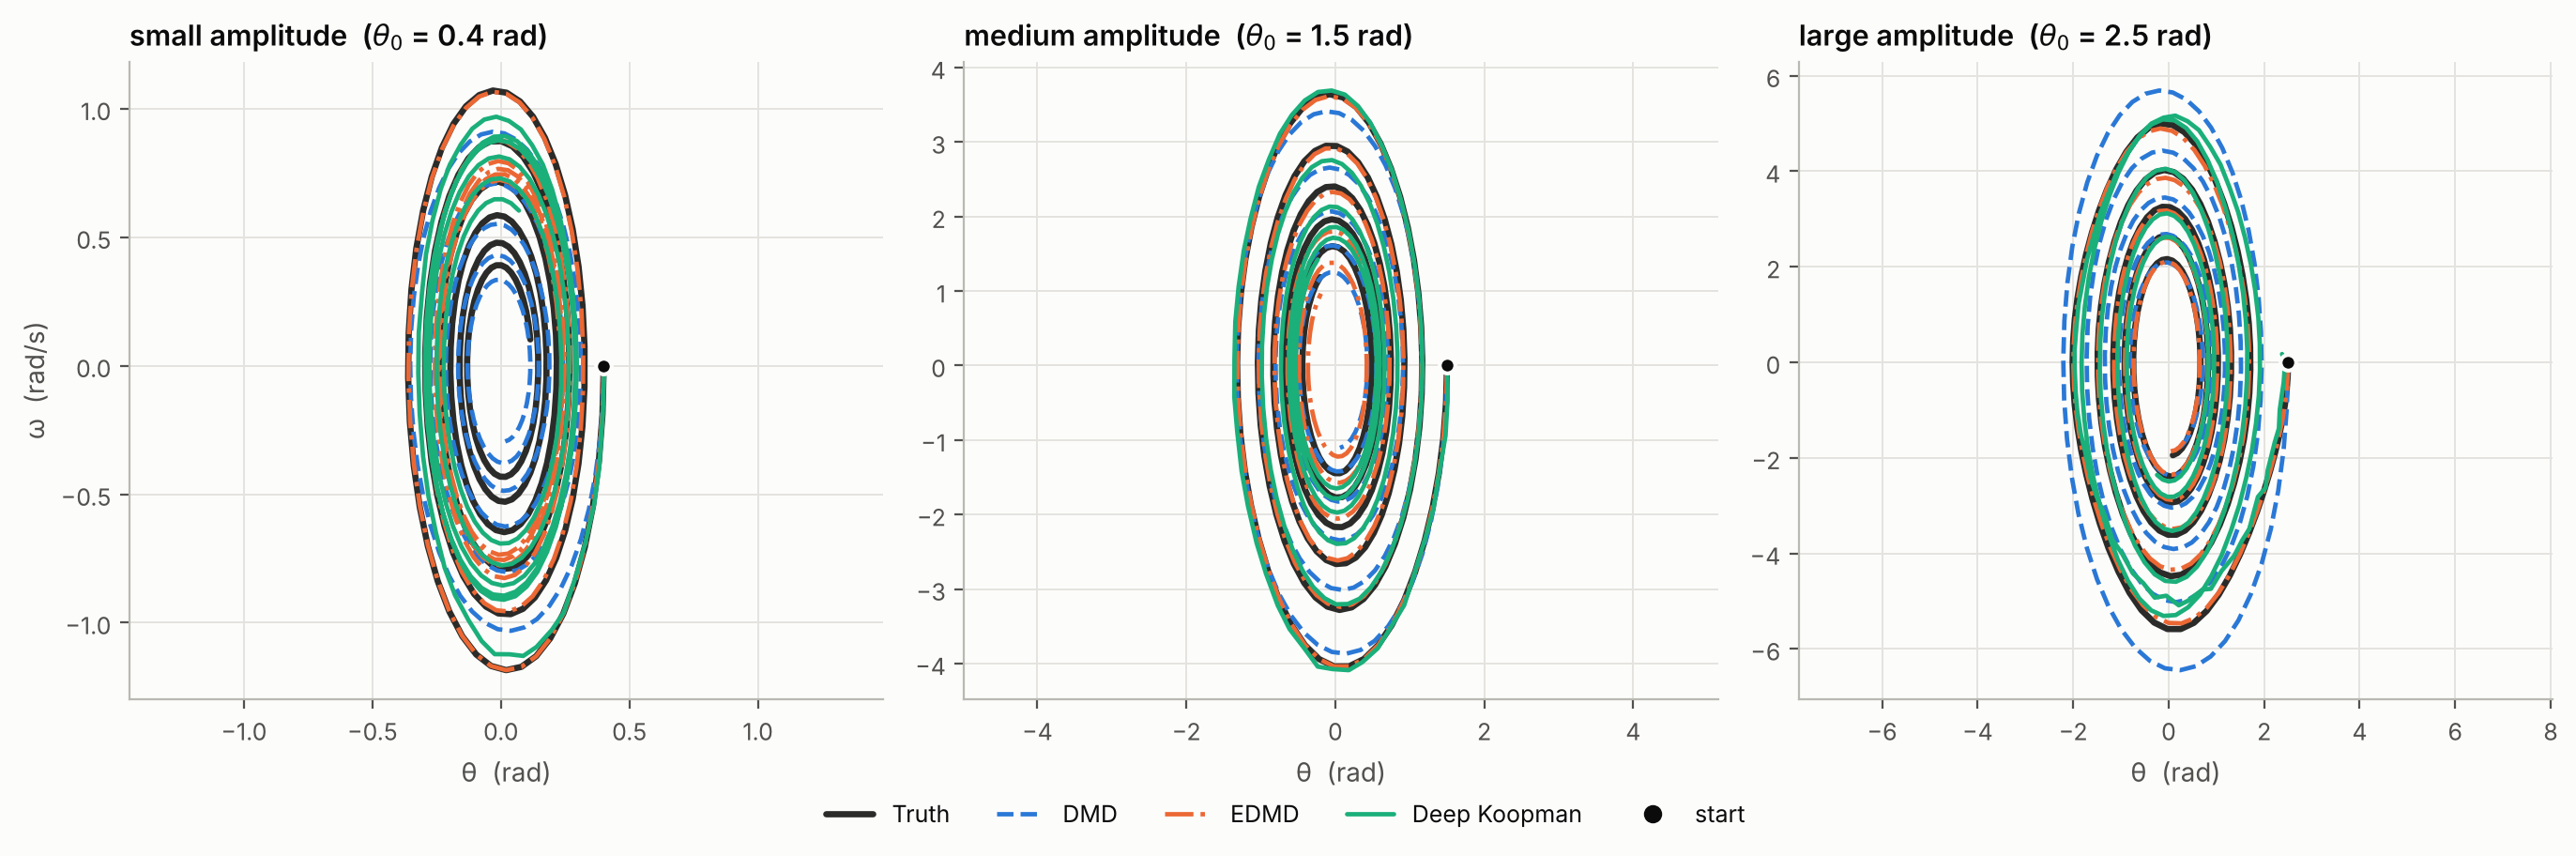
\includegraphics[width=.85\textwidth]{pendulum_phase_portraits.png}
\caption{Phase portraits of three releases (small, medium and large amplitude).}\label{fig:phase}
\end{figure}
\begin{figure}[H]\centering
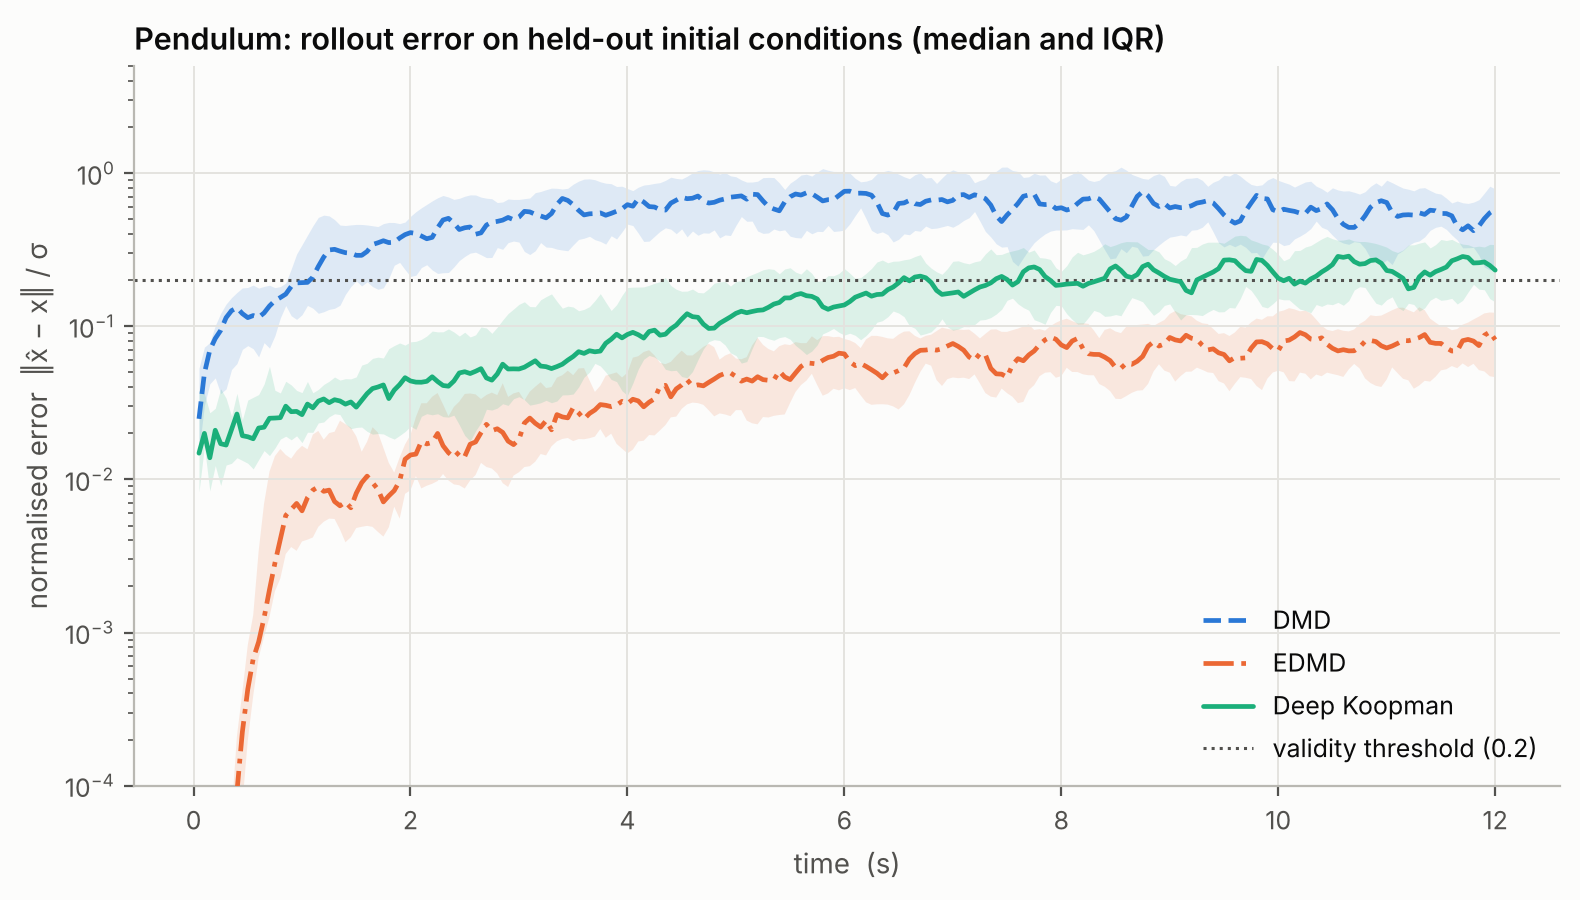
\includegraphics[width=.8\textwidth]{pendulum_error_curves.png}
\caption{Rollout error versus time (median and inter-quartile range) on the test set.}\label{fig:perr}
\end{figure}
\begin{figure}[H]\centering
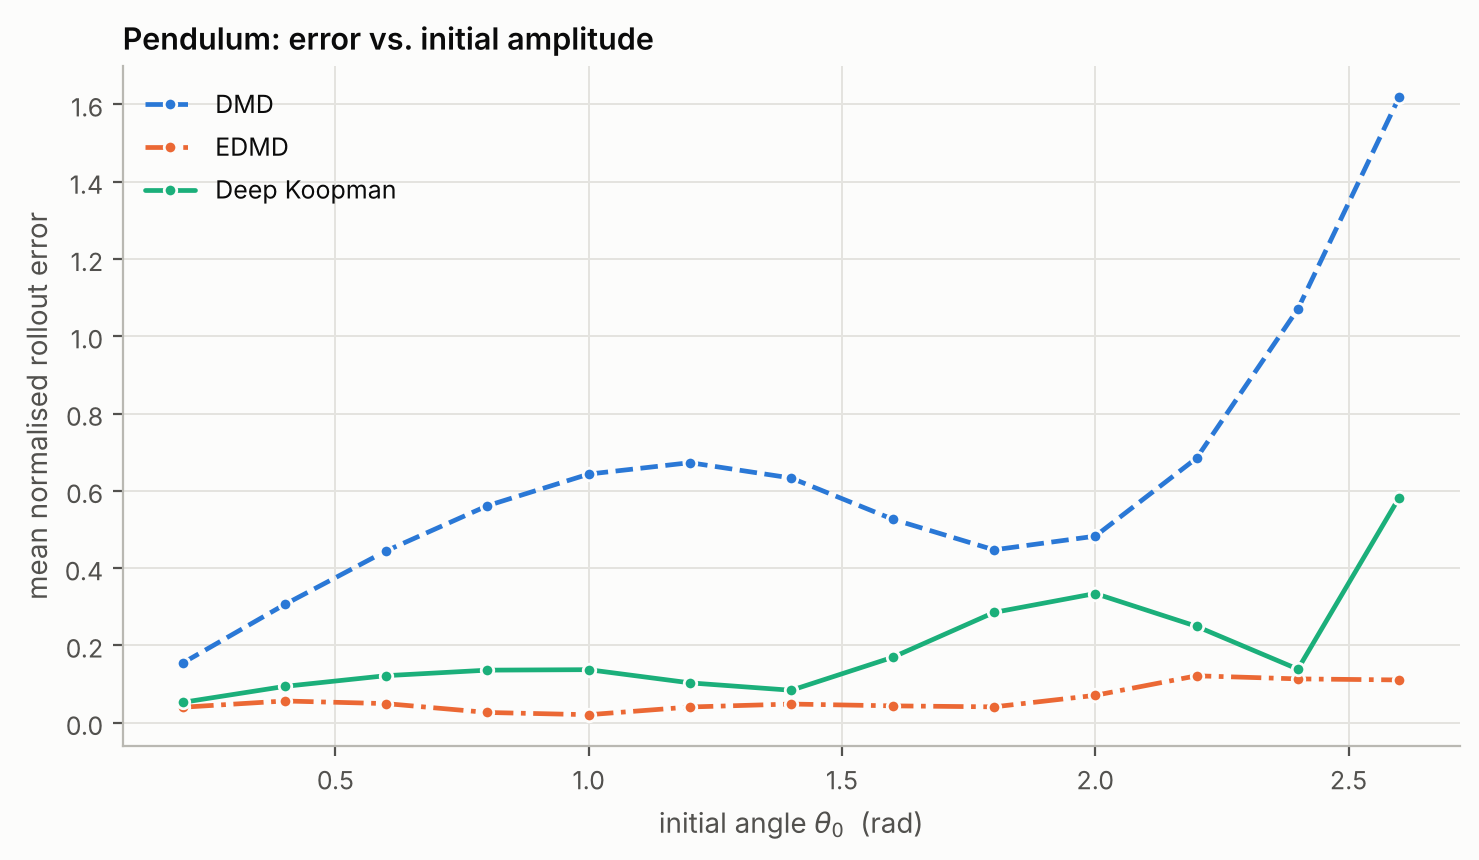
\includegraphics[width=.8\textwidth]{pendulum_error_vs_amplitude.png}
\caption{Mean rollout error versus initial amplitude.}\label{fig:amp}
\end{figure}

\subsection{Lorenz attractor}
Lorenz is chaotic, so every method fails within a fraction of a Lyapunov time (Table~\ref{tab:lor}); this is expected rather than a
bug, since a finite-dimensional linear model of a chaotic flow cannot track a trajectory over long horizons. EDMD (degree
\lorEDMDDegree{} polynomials, \lorEDMDFeatures{} observables) has the best one-step accuracy and the best mean error, yet a short valid time
($0.2$ Lyapunov times). Deep Koopman has the longest valid time ($0.44$) but a large one-step RMSE, because a single step
includes the autoencoder reconstruction error. Figure~\ref{fig:ladder} separates the sources of error for Deep Koopman: the
reconstruction alone is small, one step roughly triples it, and after one Lyapunov time the prediction error is $\approx0.6$.

\begin{table}[H]
\centering\footnotesize
\caption{Lorenz, \lorNStarts{} test initial states. Times in Lyapunov times.}\label{tab:lor}
\begin{tabular}{lrrrrr}
\toprule
Method & mean error & median valid & mean valid & never exceeded & one-step RMSE \\
\midrule
\lorenzTableRows
\bottomrule
\end{tabular}
\end{table}

\begin{table}[H]
\centering\footnotesize
\caption{Deep Koopman normalised error on Lorenz at increasing horizons.}\label{tab:ladder}
\begin{tabular}{lr}
\toprule
Horizon & normalised error \\
\midrule
\ladderTableRows
\bottomrule
\end{tabular}
\end{table}

\begin{figure}[H]\centering
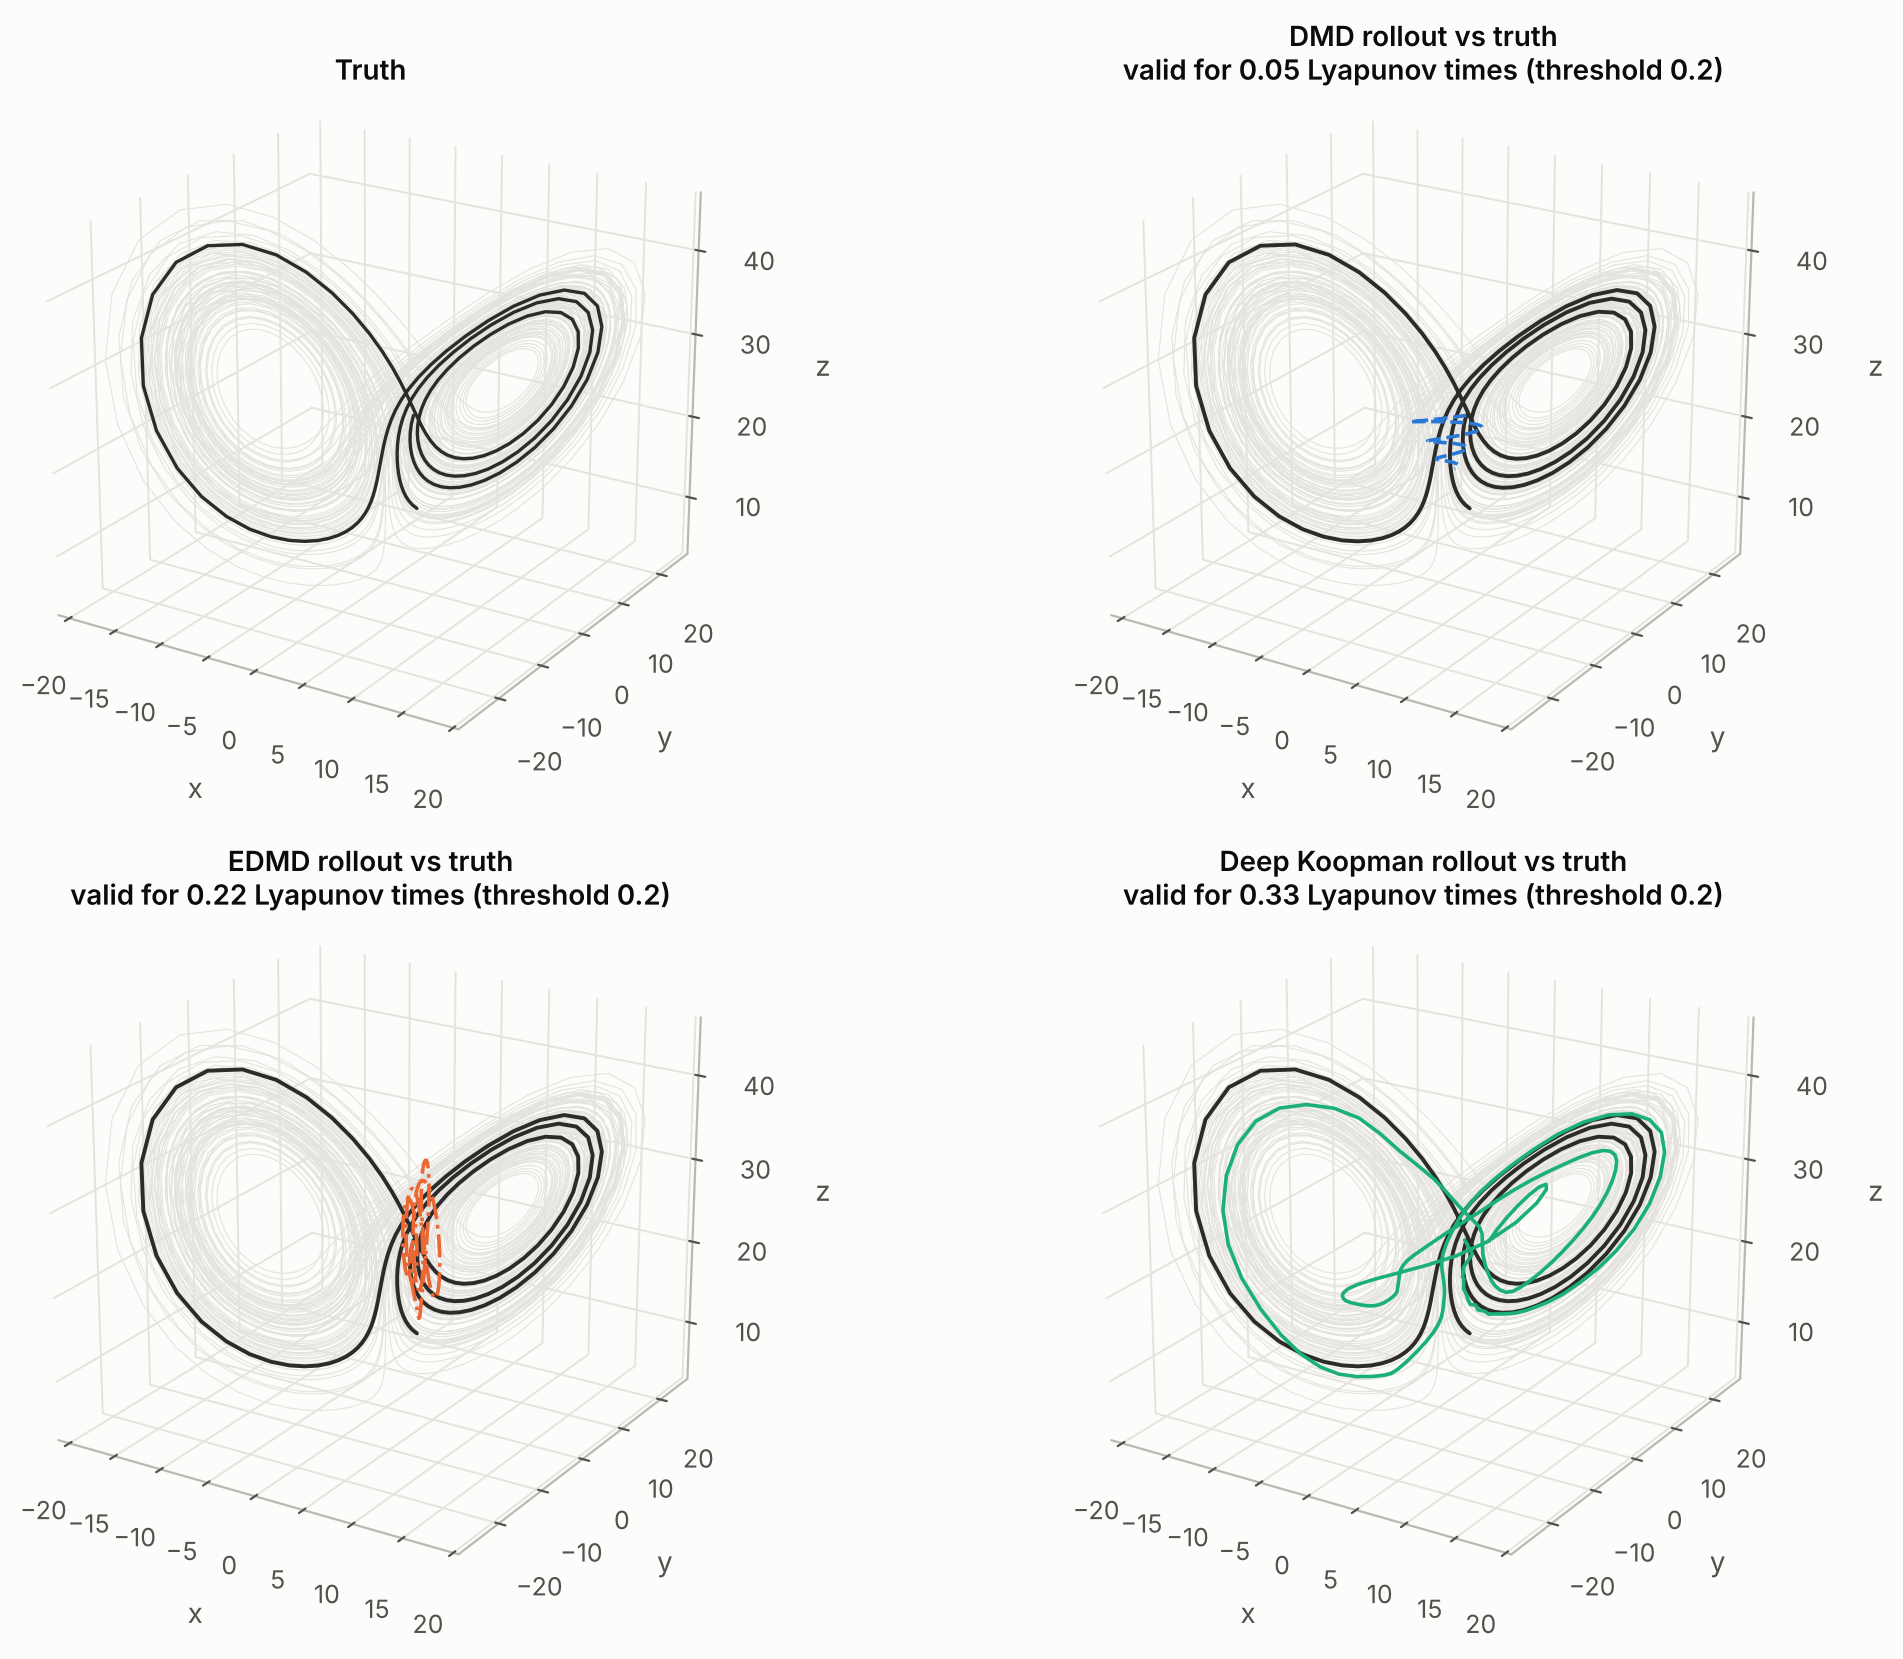
\includegraphics[width=.95\textwidth]{lorenz_attractor_comparison.png}
\caption{One test trajectory and each model's rollout from its initial state.}\label{fig:att}
\end{figure}
\begin{figure}[H]\centering
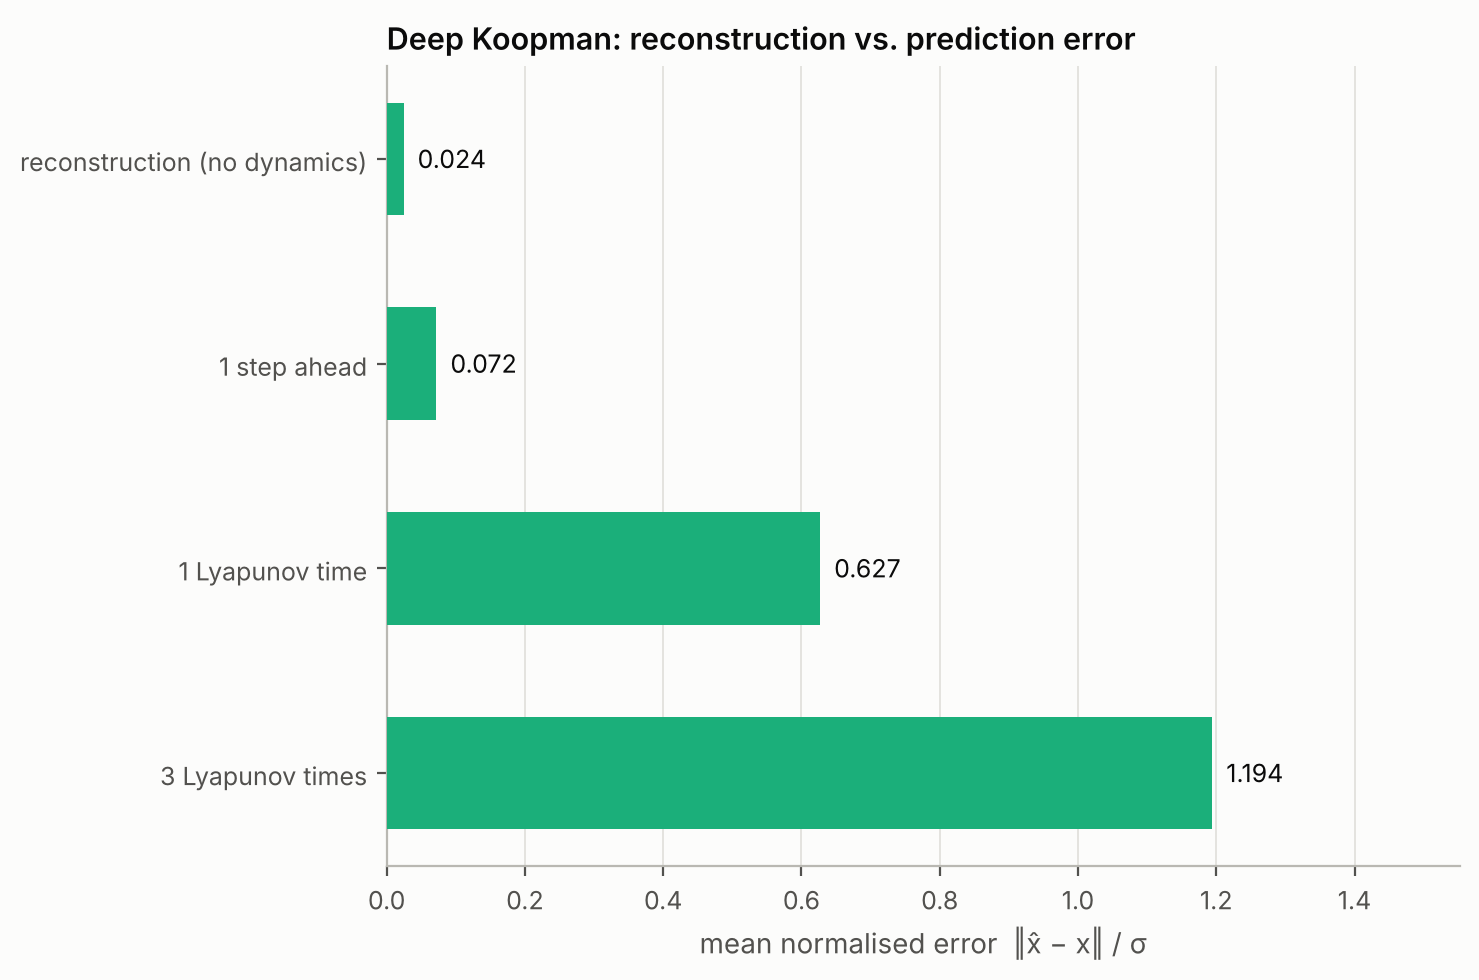
\includegraphics[width=.8\textwidth]{lorenz_reconstruction_vs_prediction.png}
\caption{Deep Koopman error ladder: reconstruction, one step, one and three Lyapunov times.}\label{fig:ladder}
\end{figure}
\begin{figure}[H]\centering
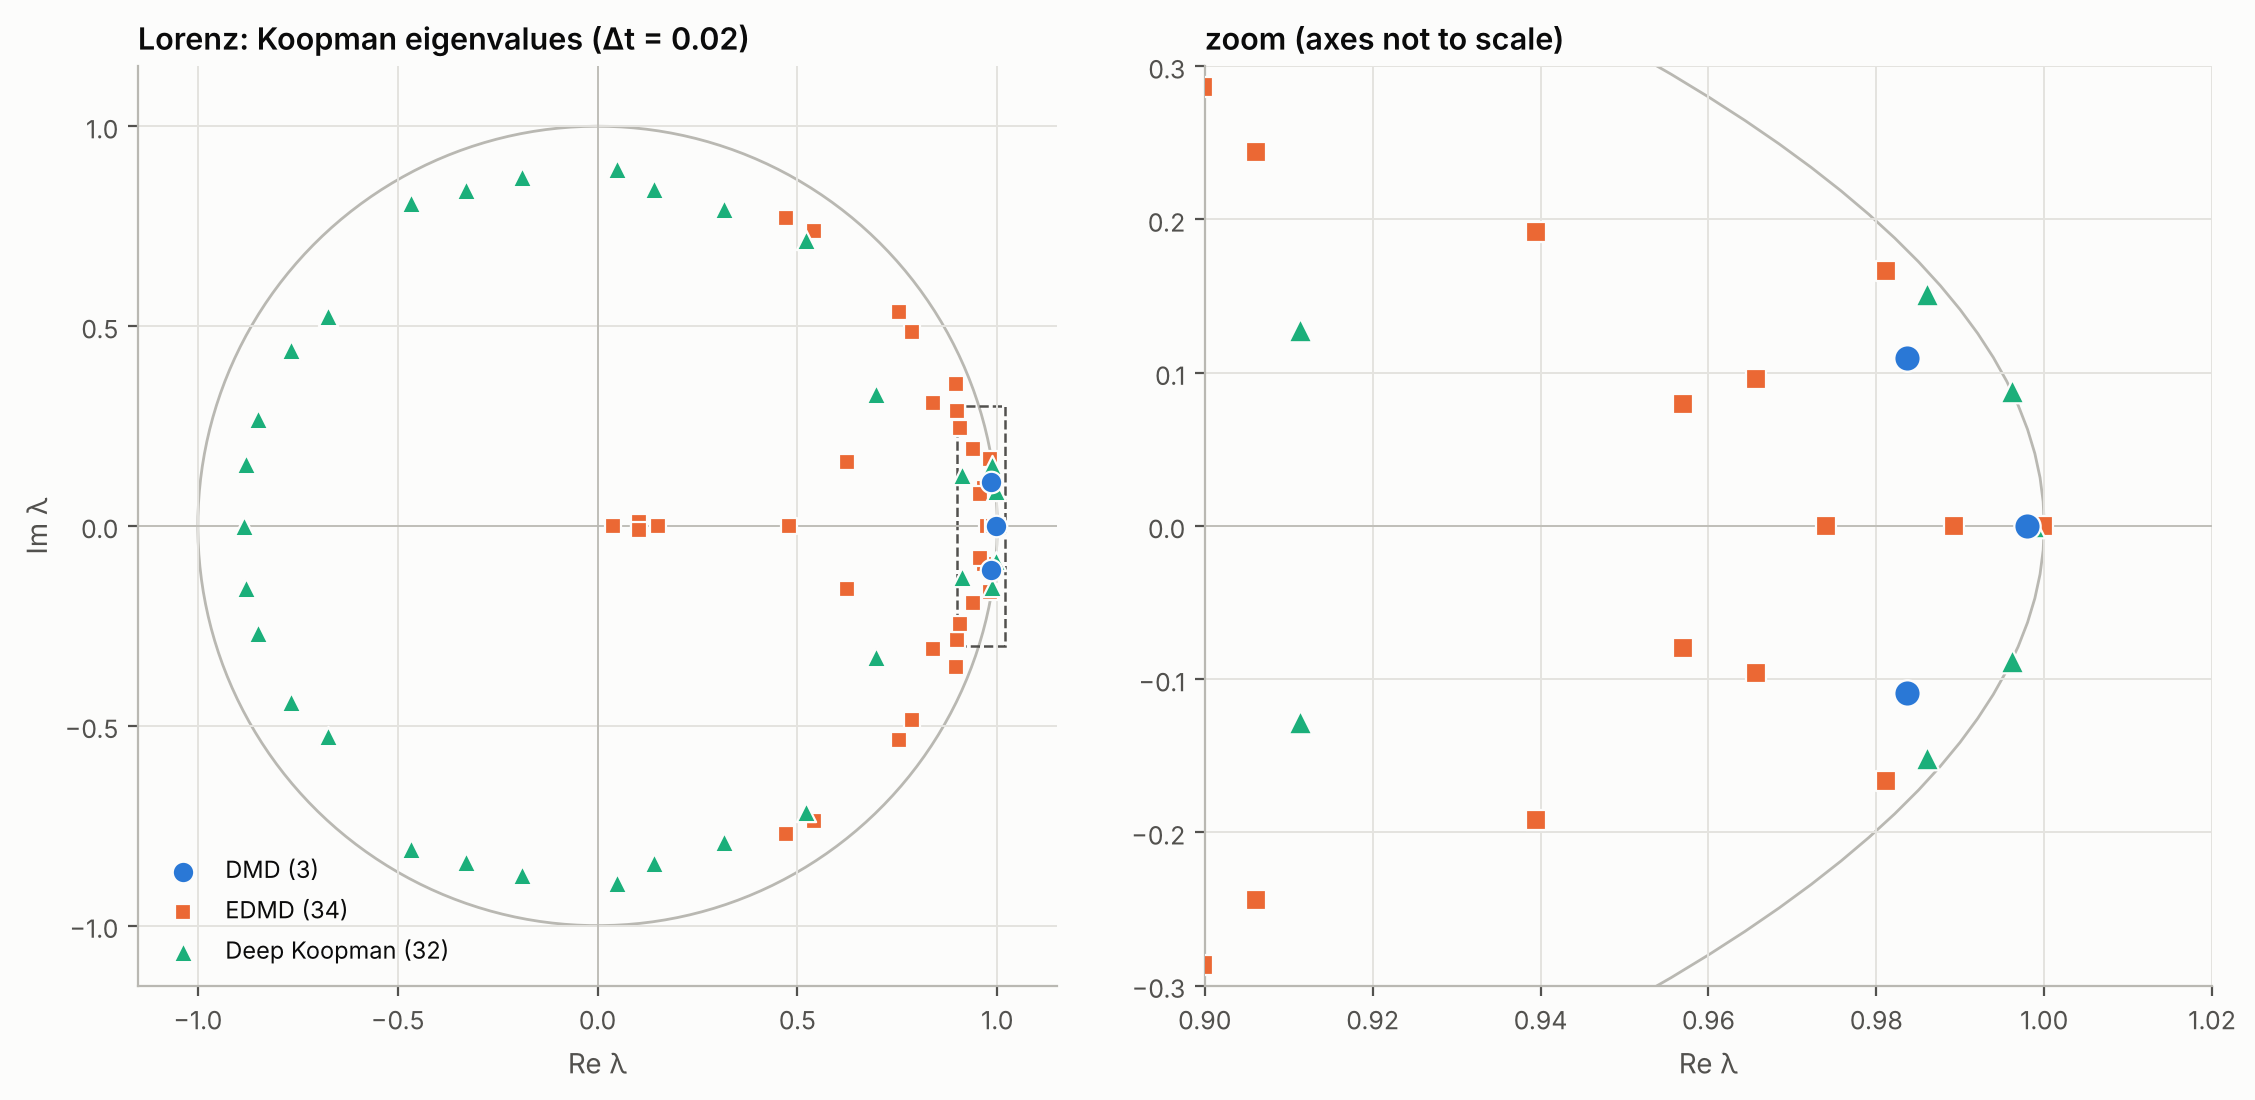
\includegraphics[width=.95\textwidth]{lorenz_spectrum.png}
\caption{Eigenvalues of the learned operators (left: unit disc; right: magnified region near $\lambda=1$).}\label{fig:spec}
\end{figure}


\subsection{Remaining figures}
\begin{figure}[H]\centering
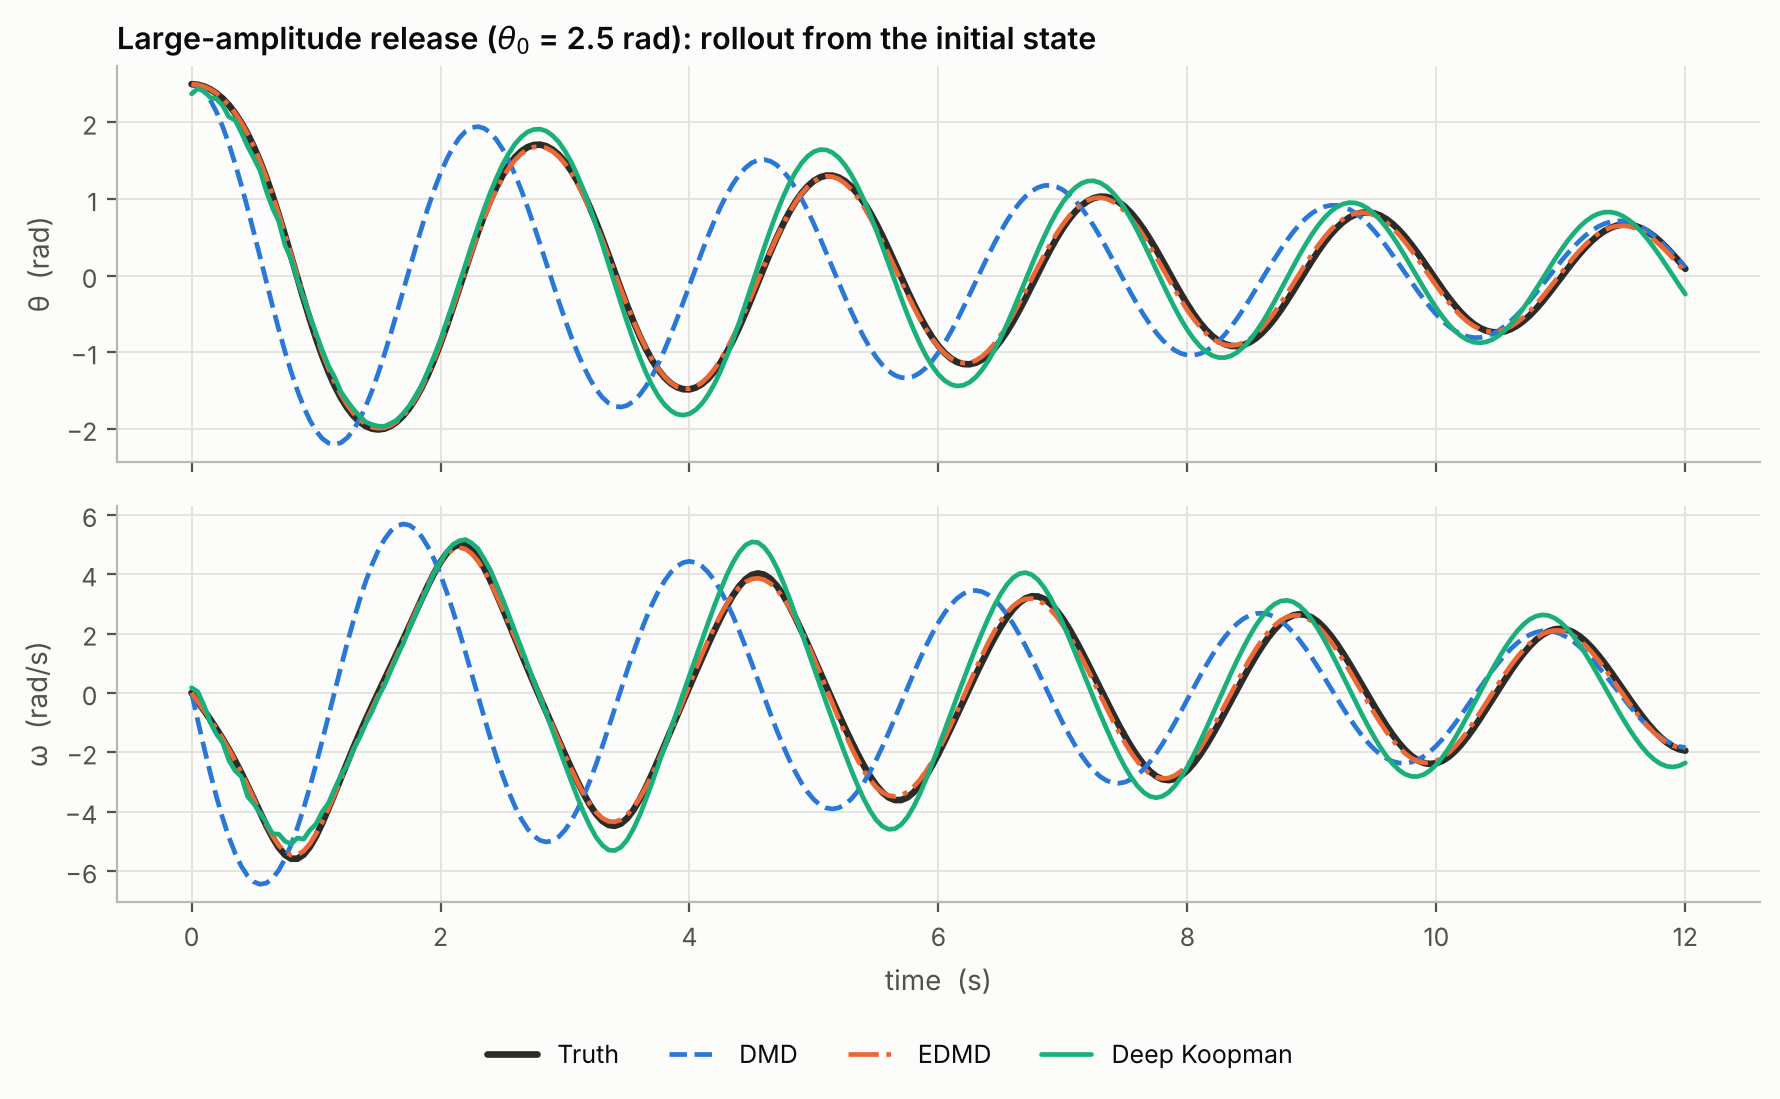
\includegraphics[width=.8\textwidth]{pendulum_time_series.png}
\caption{Time series of the large-amplitude release.}
\end{figure}
\begin{figure}[H]\centering
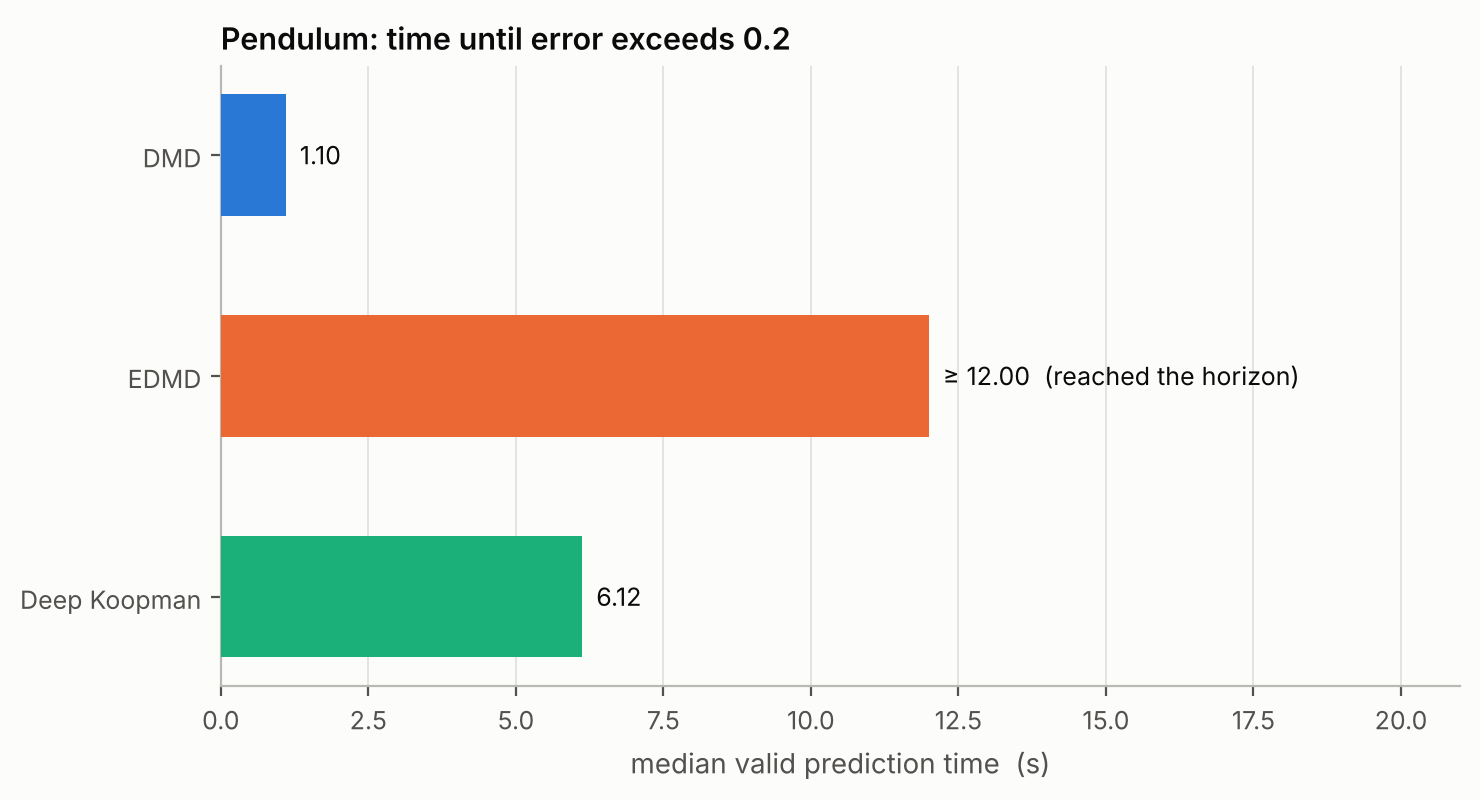
\includegraphics[width=.6\textwidth]{pendulum_valid_time.png}
\caption{Pendulum valid prediction time (the EDMD bar reached the horizon).}
\end{figure}
\begin{figure}[H]\centering
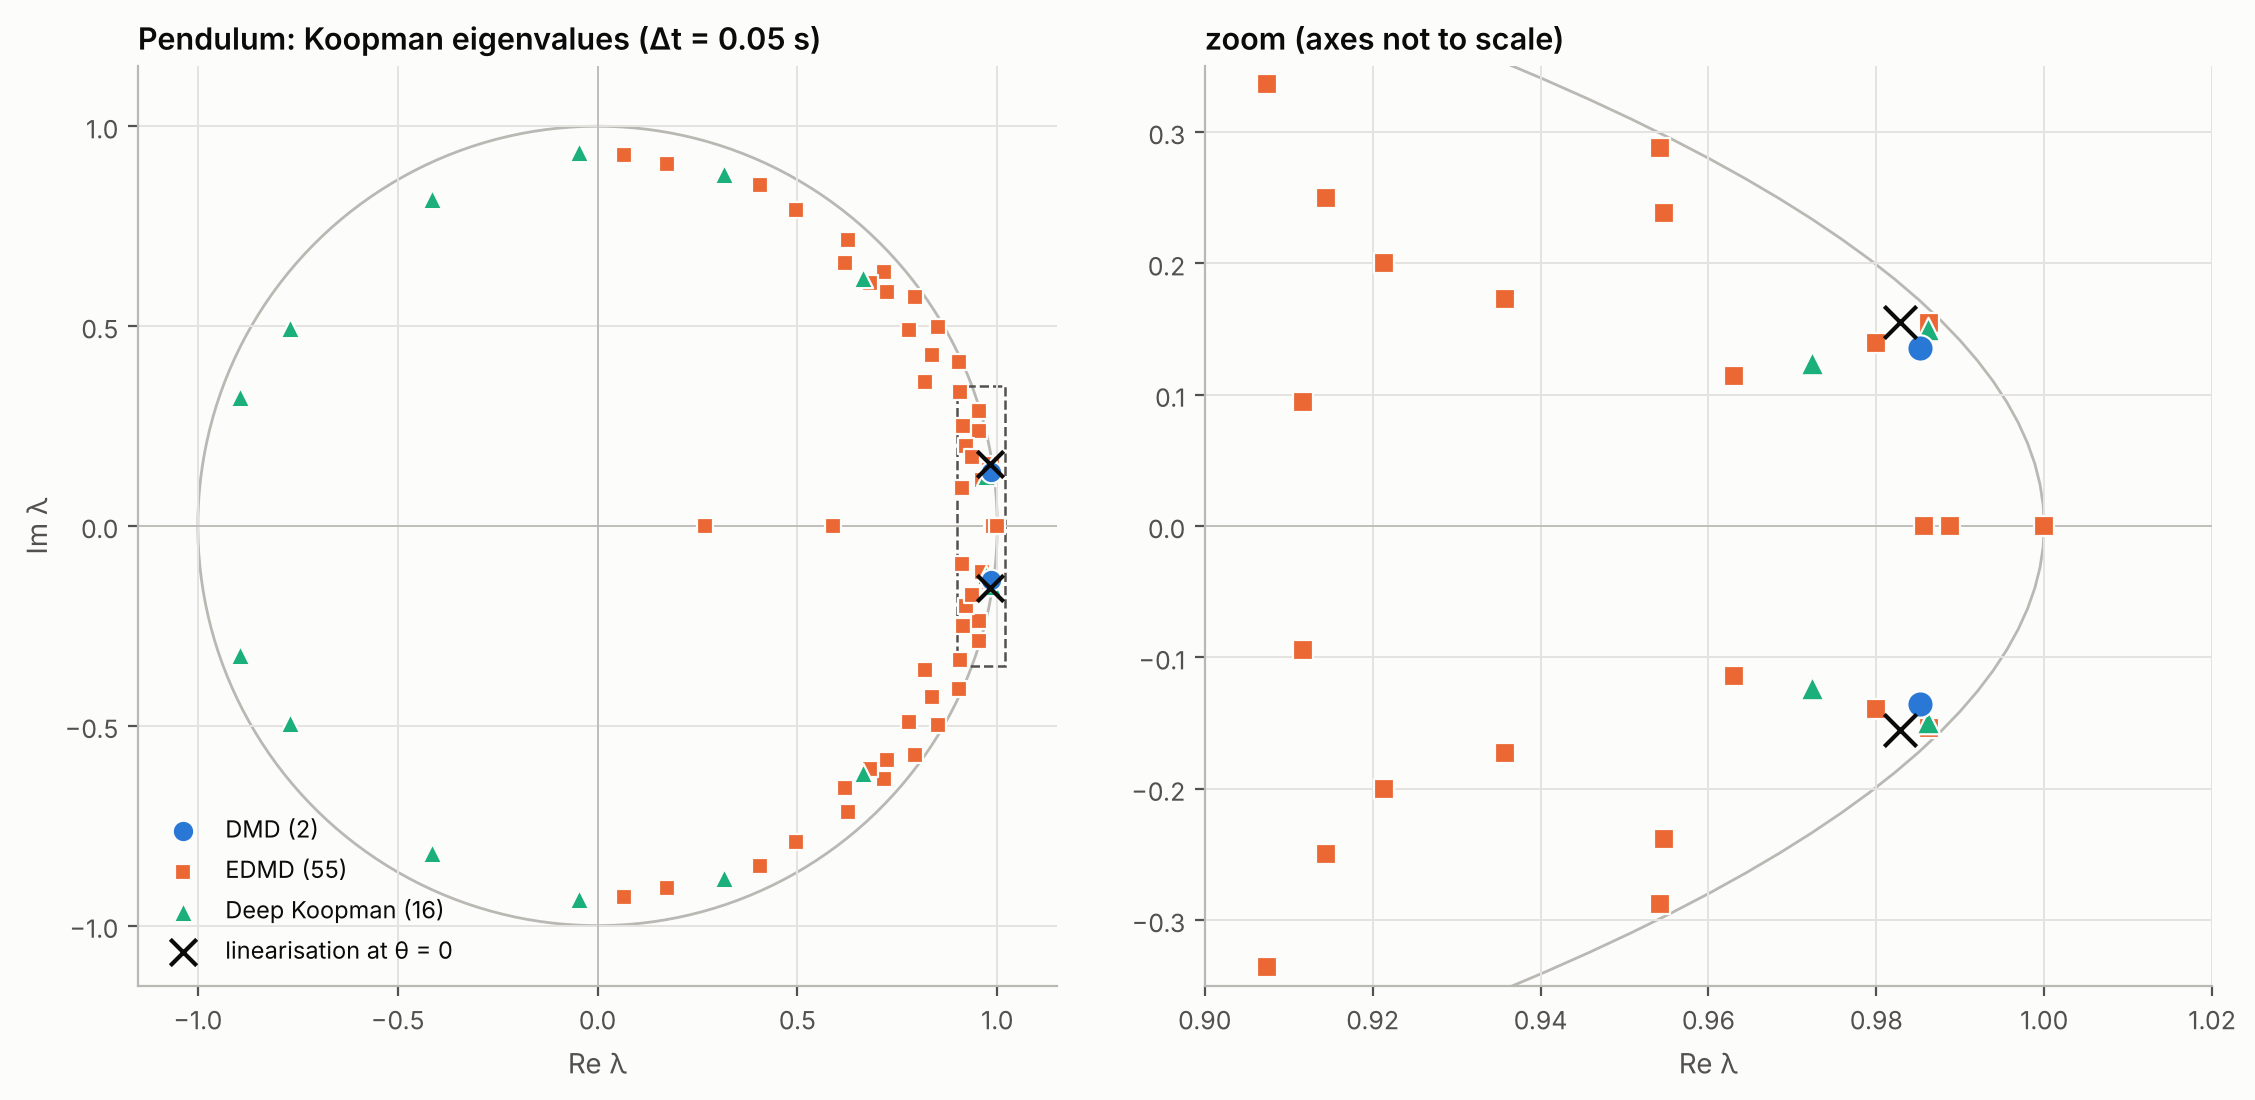
\includegraphics[width=.75\textwidth]{pendulum_spectrum.png}
\caption{Pendulum operator spectra.}
\end{figure}
\begin{figure}[H]\centering
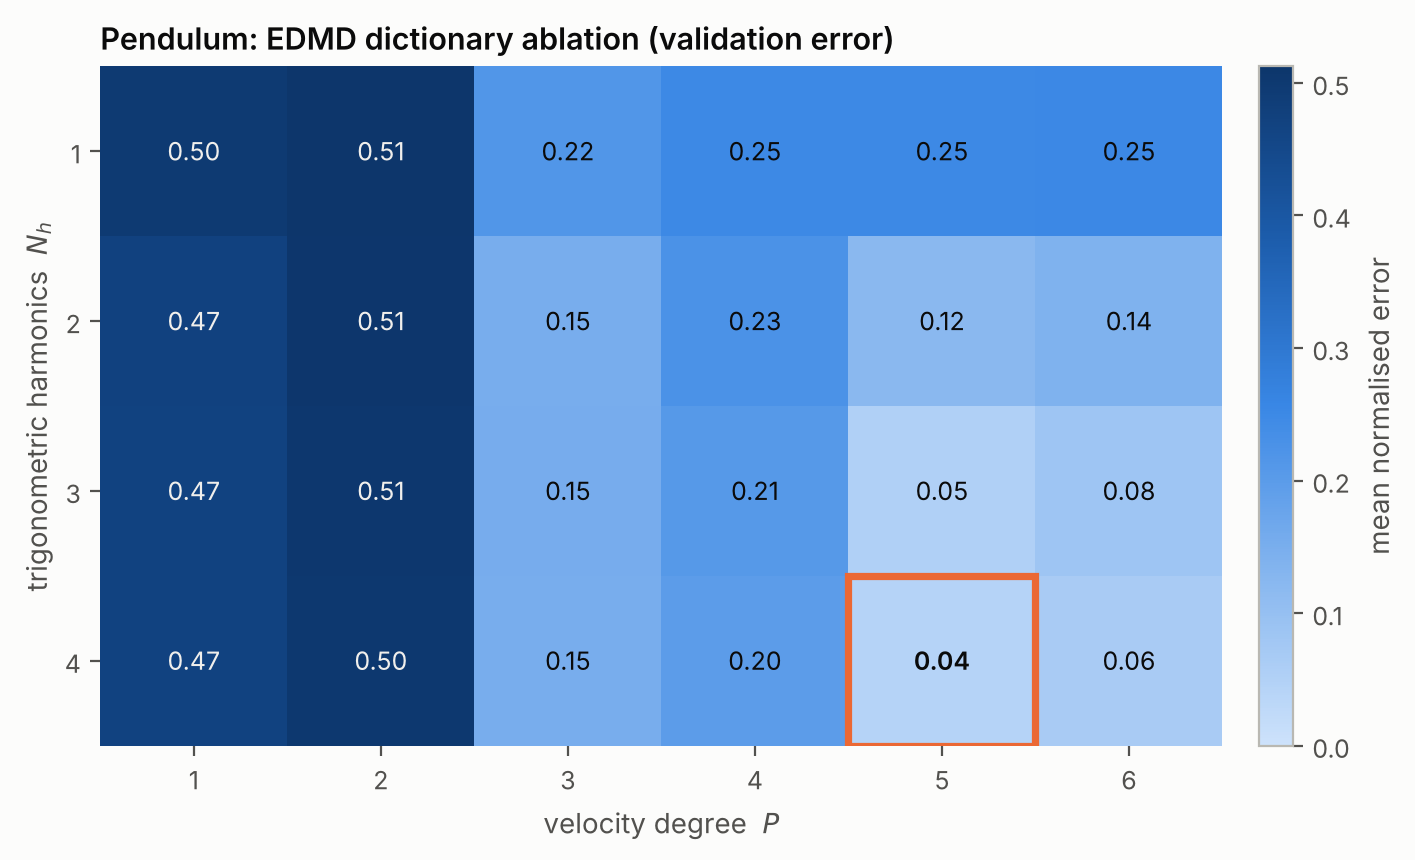
\includegraphics[width=.8\textwidth]{pendulum_edmd_ablation.png}
\caption{EDMD dictionary ablation on validation data.}
\end{figure}
\begin{figure}[H]\centering
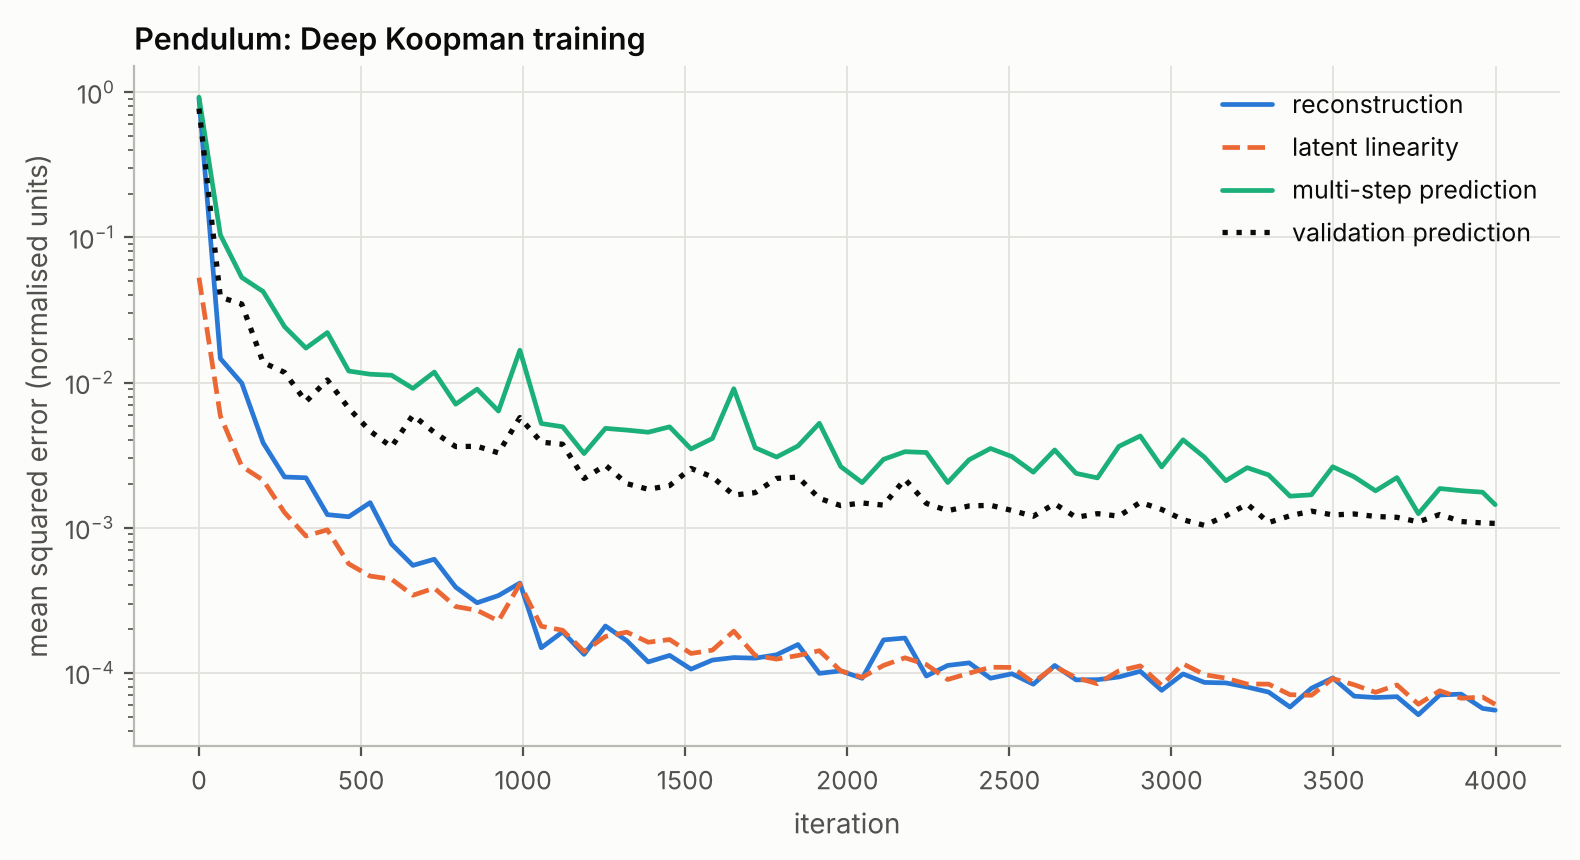
\includegraphics[width=.8\textwidth]{pendulum_training.png}
\caption{Deep Koopman training history (pendulum).}
\end{figure}
\begin{figure}[H]\centering
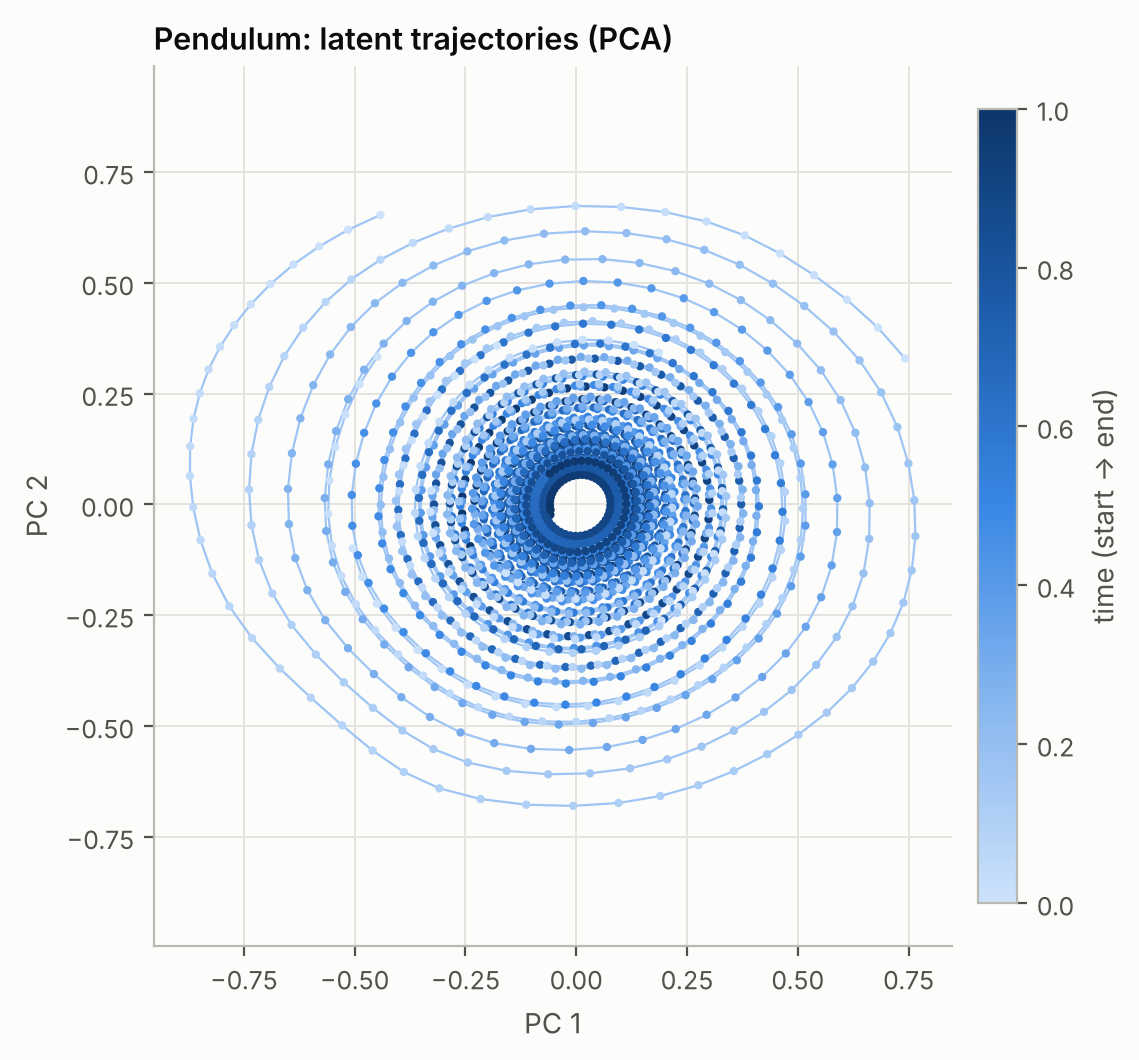
\includegraphics[width=.6\textwidth]{pendulum_latent.png}
\caption{Pendulum latent trajectories (PCA).}
\end{figure}
\begin{figure}[H]\centering
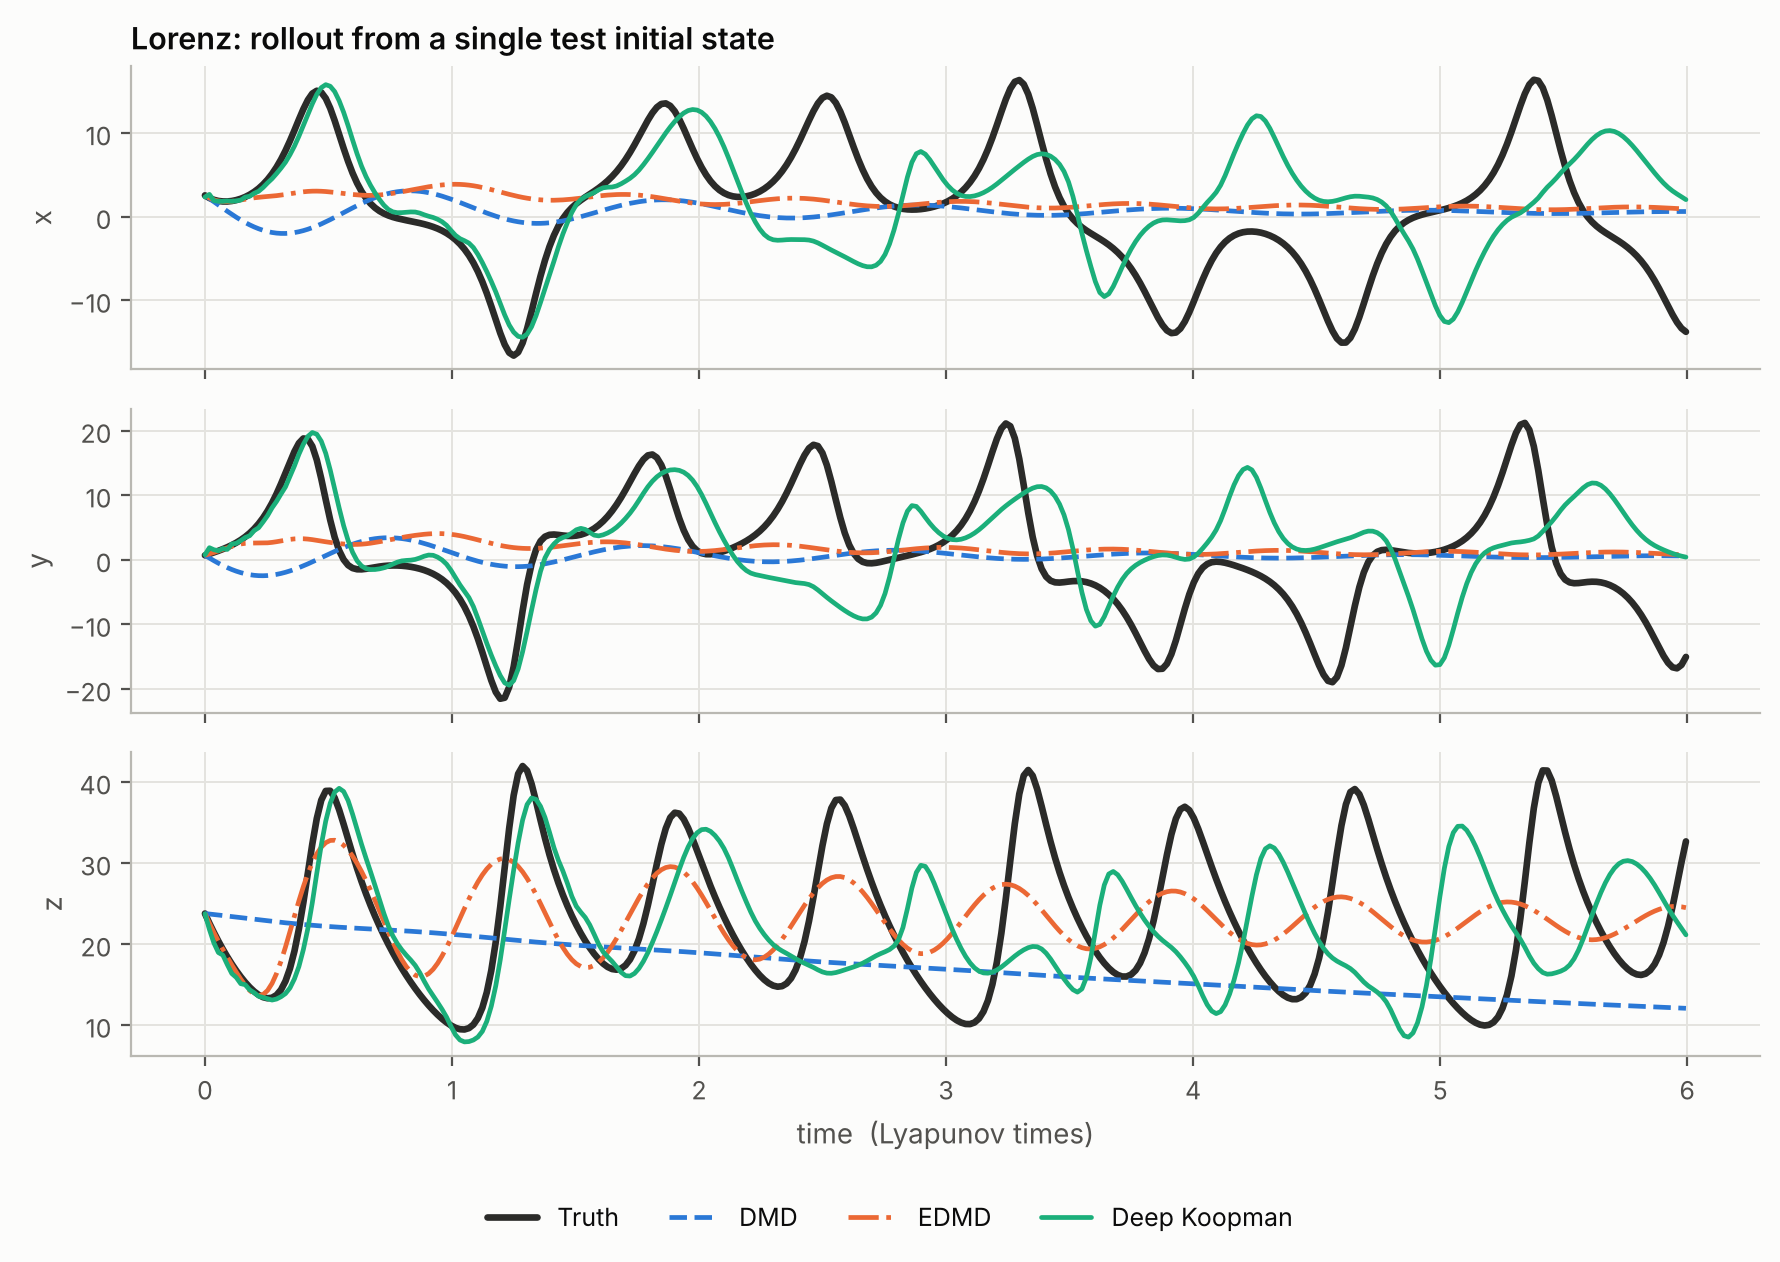
\includegraphics[width=.85\textwidth]{lorenz_time_series.png}
\caption{Lorenz time series of one test trajectory.}
\end{figure}
\begin{figure}[H]\centering
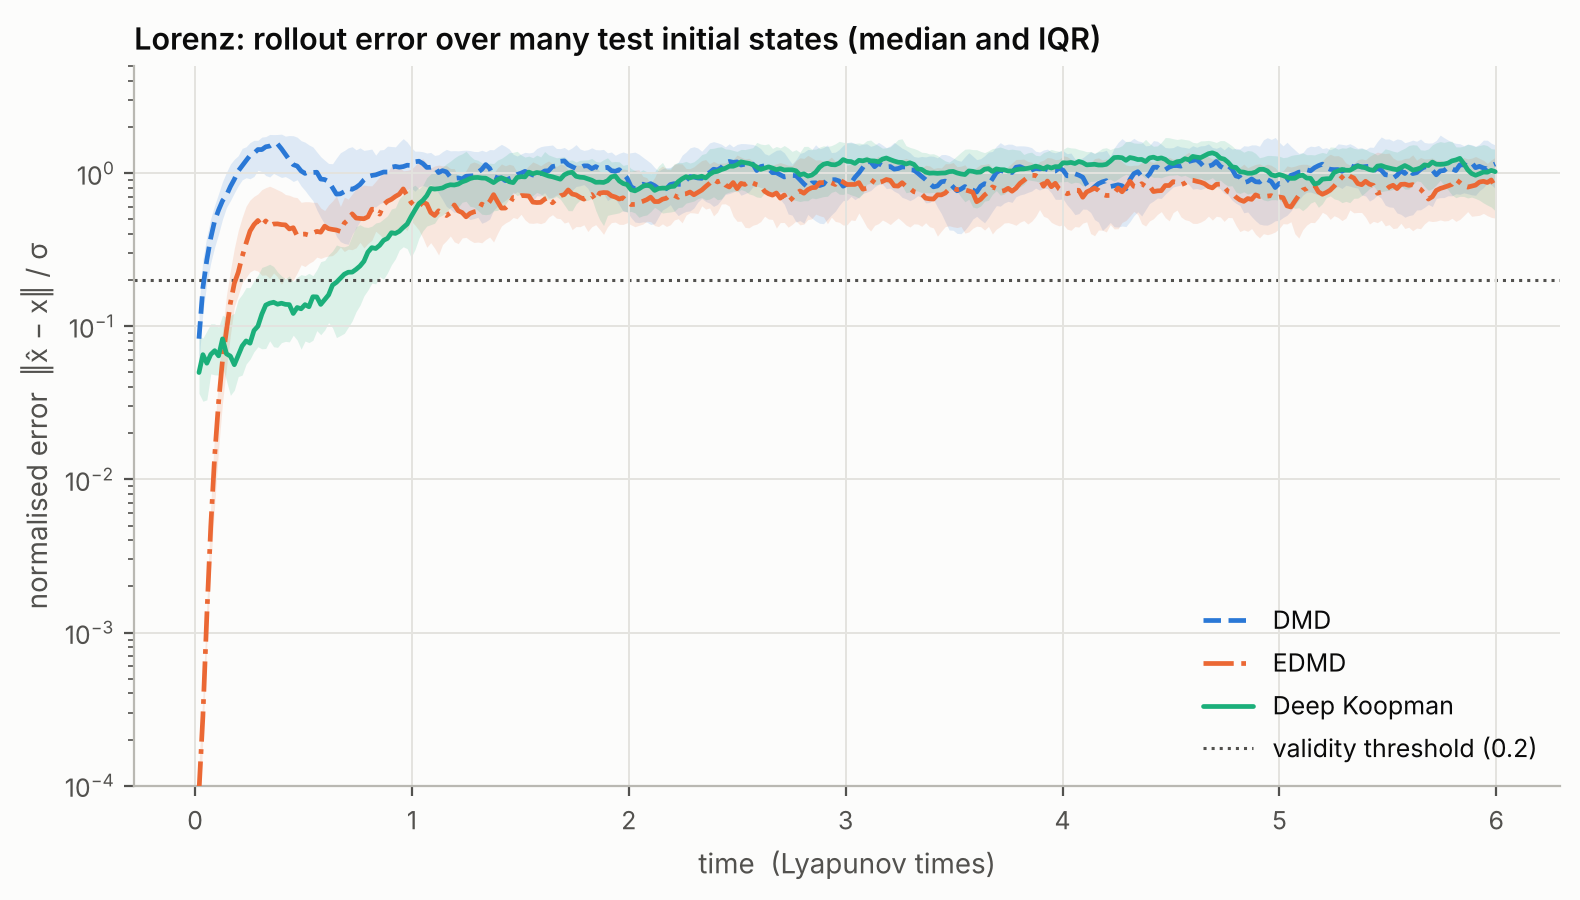
\includegraphics[width=.8\textwidth]{lorenz_error_curves.png}
\caption{Lorenz rollout error versus time.}
\end{figure}
\begin{figure}[H]\centering
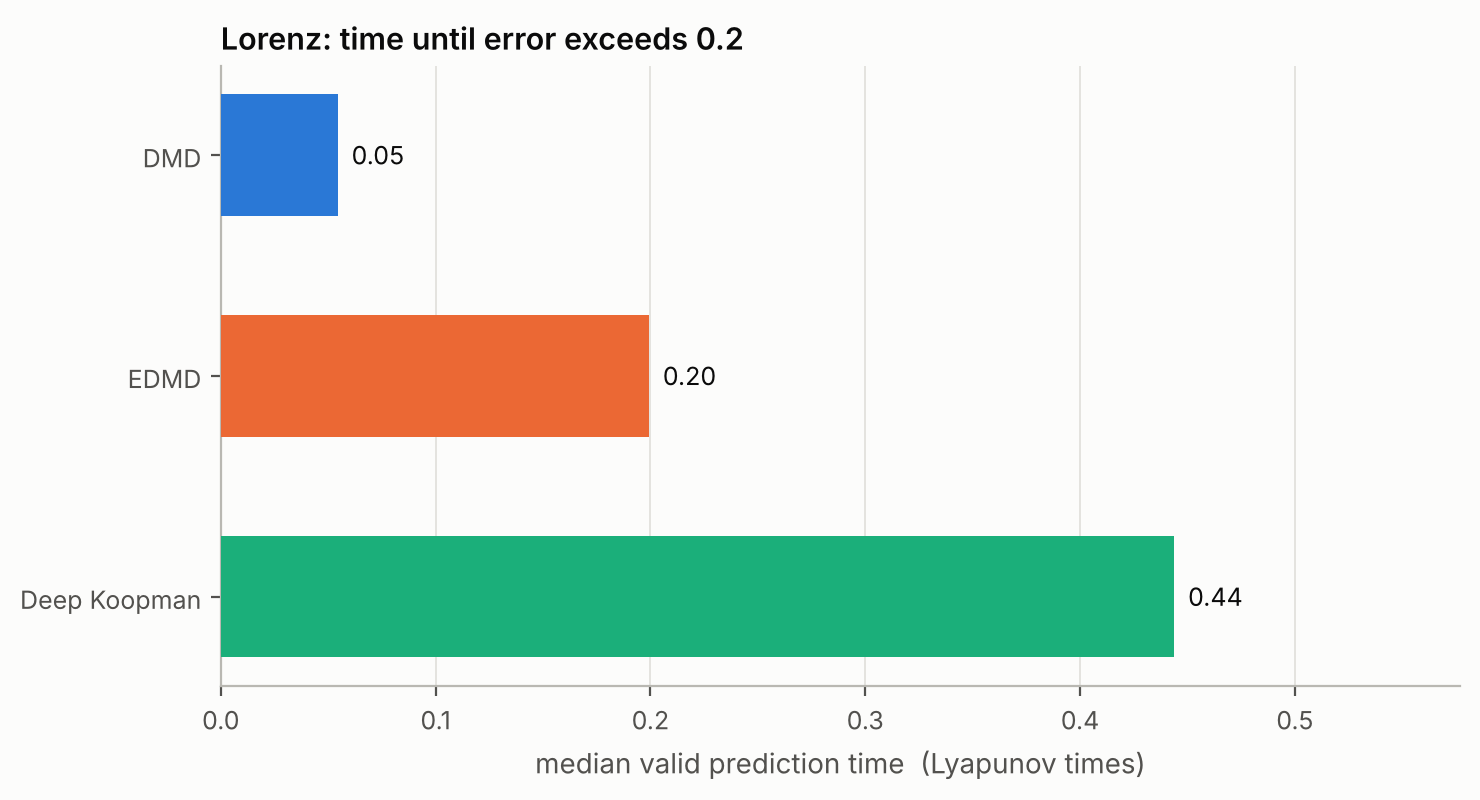
\includegraphics[width=.6\textwidth]{lorenz_valid_time.png}
\caption{Lorenz valid prediction time.}
\end{figure}
\begin{figure}[H]\centering
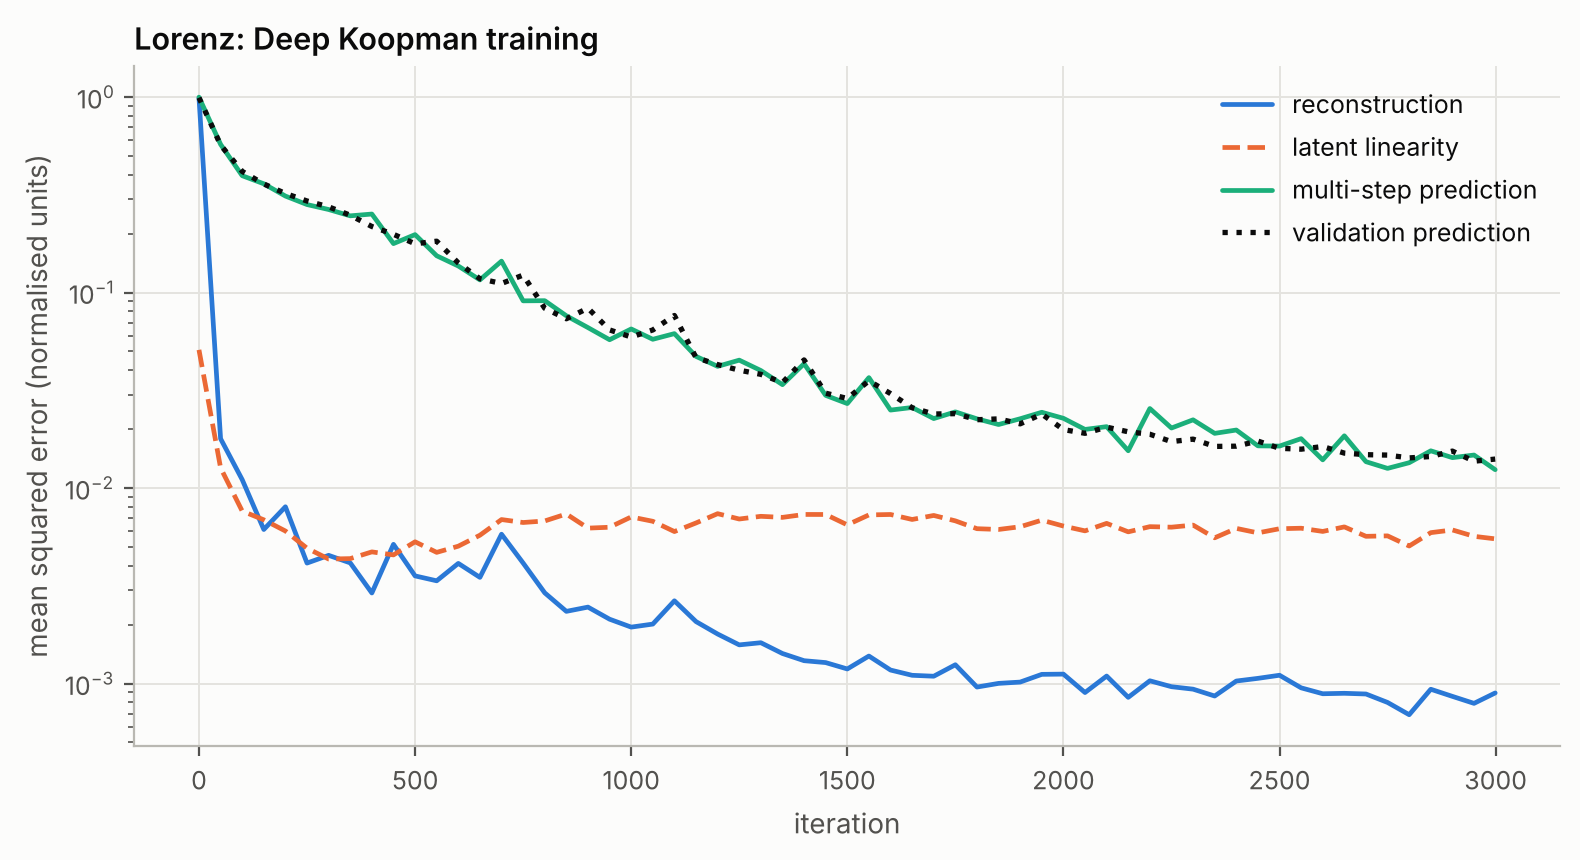
\includegraphics[width=.8\textwidth]{lorenz_training.png}
\caption{Deep Koopman training history (Lorenz).}
\end{figure}
\begin{figure}[H]\centering
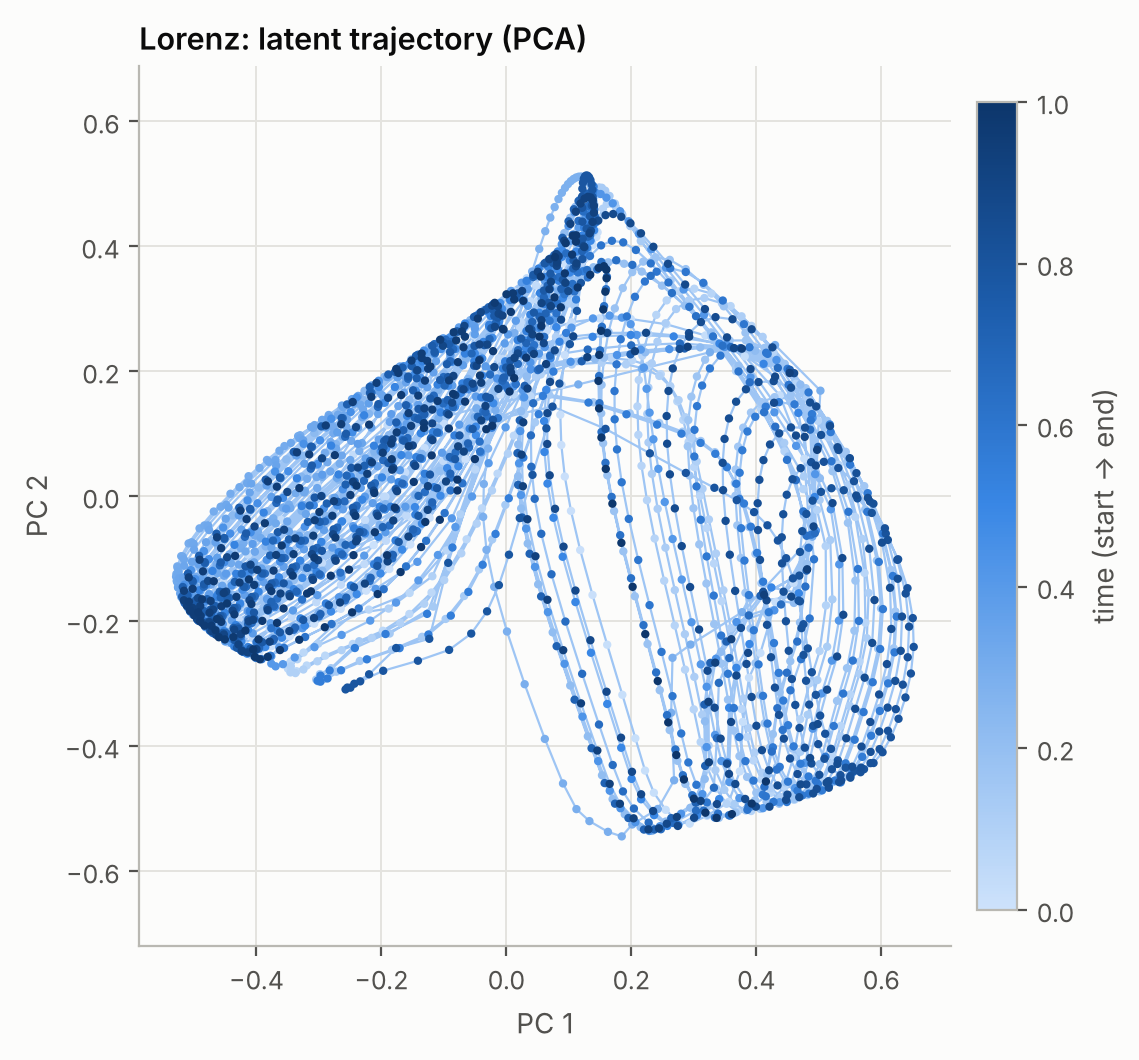
\includegraphics[width=.6\textwidth]{lorenz_latent.png}
\caption{Lorenz latent trajectories (PCA).}
\end{figure}

%% ====================================================================================
\section{How to read each figure}
%% ====================================================================================

All figures are in \code{results/figures/}. Colours are colour-blind safe and every method also has its own line style.
\begin{description}
\item[Phase portraits.] Each panel shows $(\theta,\omega)$ for one release. The truth (dark) spirals into the origin because of
damping; a model is good when its curve lies on the truth. DMD's curve decays at the wrong rate/frequency for large amplitude.
\item[Time series.] $\theta(t)$ and $\omega(t)$ for the large release. Look for phase drift: a model whose peaks gradually
move away from the truth has the wrong frequency.
\item[Error curves.] Log-scale normalised error versus time; line = median, band = inter-quartile range, dashed line = the $0.2$
validity threshold. The time where a curve crosses the dashed line is that method's valid prediction time.
\item[Valid-time bars.] Median valid time per method. A bar labelled ``$\geq$ value'' reached the horizon, so the number is a
lower bound.
\item[Error versus amplitude.] Mean error per initial amplitude $\theta_0$; a rising curve means the method degrades in the
nonlinear regime.
\item[Spectrum.] Eigenvalues of the learned discrete operators in the complex plane; the circle is $|\lambda|=1$. Points inside
the circle decay, points on it oscillate indefinitely. The reference (linearised pendulum) is the target near $\lambda=1$; the
right panel magnifies that region and its axes are not to scale.
\item[Training history.] Deep Koopman loss terms (reconstruction, linearity, prediction) and validation prediction error versus
iteration; all should decrease, and a growing validation curve signals overfitting.
\item[Latent PCA.] Latent trajectories projected on two principal components; for a pendulum these should be smooth spirals.
\item[EDMD ablation.] Validation error as a function of harmonics $N_h$ and velocity degree $P$; the outlined cell is the choice.
\item[Lorenz attractor comparison.] Four 3D panels (truth, DMD, EDMD, Deep Koopman); the grey background is the attractor, the
dark curve the truth over the plotted window, the coloured curve a rollout. A rollout that collapses to a point or small loop
has lost the dynamics; the panel title gives the valid time.
\item[Lorenz error ladder.] Deep Koopman error for reconstruction, one step, one and three Lyapunov times: it shows whether
the error comes from the autoencoder or from propagating the dynamics.
\end{description}


%% ====================================================================================
\section{Limitations and honest caveats}
%% ====================================================================================

\begin{itemize}
\item \textbf{Single seed.} All numbers come from one seed (0); differences between methods on Lorenz are small and might change
with other seeds. No confidence intervals were computed.
\item \textbf{Deep Koopman tuning.} Its hyper-parameters were chosen on a modest validation grid, not exhaustively; a larger
search might improve it.
\item \textbf{Lorenz is hard for any finite linear Koopman model.} Valid times below half a Lyapunov time are a fundamental
limit of this approach, not only of this implementation. The Deep Koopman eigenvalues were slightly outside the unit circle
(radius $\approx1.018$) and a post-hoc rescaling was used, selected on validation data only.
\item \textbf{Capped pendulum EDMD result.} The EDMD median valid time is limited by the $12\,$s horizon, so the true value is
larger.
\item \textbf{Dictionary parity effect.} The EDMD validation error depends on whether the velocity degree $P$ is odd or even
(see the ablation figure); I observed it but did not investigate its cause.
\item \textbf{One-step error of Deep Koopman} is dominated by the autoencoder's reconstruction error.
\end{itemize}


%% ====================================================================================
\section{Reproducing the results}
%% ====================================================================================
\begin{verbatim}
pip install -r requirements.txt
pytest                      # unit + smoke tests
python main.py              # both experiments -> results/
python main.py --quick      # a few-seconds smoke run
python report/make_tables.py
cd report && pdflatex koopman_report.tex      # rebuild this report
\end{verbatim}

\begin{thebibliography}{9}
\bibitem{Koopman1931} B.\,O.~Koopman, Hamiltonian systems and transformation in Hilbert space,
  \emph{Proc.\ Natl.\ Acad.\ Sci.\ USA} \textbf{17}(5), 315--318 (1931).
\bibitem{Schmid2010} P.\,J.~Schmid, Dynamic mode decomposition of numerical and experimental data,
  \emph{J.\ Fluid Mech.} \textbf{656}, 5--28 (2010).
\bibitem{Tu2014} J.\,H.~Tu, C.\,W.~Rowley, D.\,M.~Luchtenburg, S.\,L.~Brunton, J.\,N.~Kutz, On dynamic mode decomposition:
  theory and applications, \emph{J.\ Comput.\ Dyn.} \textbf{1}(2), 391--421 (2014).
\bibitem{Williams2015} M.\,O.~Williams, I.\,G.~Kevrekidis, C.\,W.~Rowley, A data-driven approximation of the Koopman operator:
  extending dynamic mode decomposition, \emph{J.\ Nonlinear Sci.} \textbf{25}(6), 1307--1346 (2015).
\bibitem{Lusch2018} B.~Lusch, J.\,N.~Kutz, S.\,L.~Brunton, Deep learning for universal linear embeddings of nonlinear dynamics,
  \emph{Nat.\ Commun.} \textbf{9}, 4950 (2018).
\bibitem{Brunton2022} S.\,L.~Brunton, M.~Budi\v{s}i\'c, E.~Kaiser, J.\,N.~Kutz, Modern Koopman theory for dynamical systems,
  \emph{SIAM Rev.} \textbf{64}(2), 229--340 (2022).
\bibitem{Dormand1980} J.\,R.~Dormand, P.\,J.~Prince, A family of embedded Runge--Kutta formulae,
  \emph{J.\ Comput.\ Appl.\ Math.} \textbf{6}(1), 19--26 (1980).
\bibitem{Lorenz1963} E.\,N.~Lorenz, Deterministic nonperiodic flow, \emph{J.\ Atmos.\ Sci.} \textbf{20}(2), 130--141 (1963).
\end{thebibliography}

\end{document}
